\documentclass[xcolor=dvipsnames]{beamer}
\usepackage{lmodern}
\usepackage[T1]{fontenc}
\usepackage[english]{babel}
\usepackage[utf8]{inputenc}

\usepackage{manfnt}
\usepackage{wasysym}
\usepackage{listings}
\usepackage{graphicx}
\usepackage{url}
\usepackage{ulem}
\usepackage{marvosym}
\usepackage{skull}
\usepackage{proof}
\usepackage{array}
\usepackage{colortbl}
\usepackage{xspace}
\setbeamertemplate{navigation symbols}{}

\title[]{{\bf Practical Concurrency Testing}}
\subtitle[]{or, \\ How I Learned to Stop Worrying and Love the Exponential Explosion}
\author[]{Ben Blum \texttt{(bblum@cs.cmu.edu)}}

\institute[]{Carnegie Mellon University}
\date[]{2018, October 17}

\setbeamertemplate{footline}{\hspace*{.5cm}\scriptsize{\insertauthor\hspace*{50pt} \hfill\insertframenumber\hspace*{.5cm}}} 

\usecolortheme{seahorse}
\usecolortheme{rose}
\useoutertheme{infolines}

\usecolortheme[named=ForestGreen]{structure}

\newcommand\noob{\mathsf{noob}}
\newcommand\gibs{\mathsf{gibs}}
\newcommand\dps{\mathsf{dps}}
\newcommand\squig\rightsquigarrow
\newcommand\Coloneqq{\mathrel{\mathop{::}}=}
\newcommand\dmg{\text{\Laserbeam}}
\newcommand\delter\delta
\newcommand\alpher\alpha
\newcommand\defnor{\text{ }|\text{ }}

\newcommand\pimp{\mathop{\supset}}
\newcommand\pand{\mathop{\wedge}}
\newcommand\por{\mathop{\vee}}
\newcommand\ptrue{\top}
\newcommand\pfalse{\bot}

\newcommand\hilight[2]{\color{#1}#2\color{black}}
\definecolor{darkorange}{RGB}{192,128,0}
\definecolor{darkblue}{RGB}{0,97,192}
\definecolor{olivegreen}{RGB}{0,128,0}
\definecolor{lavender}{RGB}{102,65,208} % (?? i don't know what happened here anymore but it looks good)
\definecolor{seafoam}{RGB}{56,158,68} % * 2/3
\definecolor{salmon}{RGB}{208,89,74} % * 7/8
\definecolor{pinkish}{RGB}{224,0,56} % * 7/8
\definecolor{goldish}{RGB}{128,96,32}
\definecolor{gray}{RGB}{128,128,128}

\definecolor{sect-quicksand}{RGB}{0,96,128}
\definecolor{sect-410}{RGB}{0,128,64}
\definecolor{sect-htm}{RGB}{128,0,64}
\definecolor{sect-pastel-quicksand}{RGB}{144,180,192}
\definecolor{sect-pastel-410}{RGB}{144,192,168}
\definecolor{sect-pastel-htm}{RGB}{192,144,168}

\begin{document}
\renewcommand{\inserttotalframenumber}{69}
\normalem
\begin{frame}
	\titlepage
\end{frame}

%%%%%%%%%%%%%%%%%%%%%%%%%%%%%%%%%%%%%%%%%%%%%%%%%%%%%%%%%%%%%%%%%%%%%%%%%%%%%%%%
%%%%%%%%%%%%%%%%%%%%%%%%%%%%%%%%%%%%%%%%%%%%%%%%%%%%%%%%%%%%%%%%%%%%%%%%%%%%%%%%
%%%%%%%%%%%%%%%%%%%%%%%%%%%%%%%%%%%%%%%%%%%%%%%%%%%%%%%%%%%%%%%%%%%%%%%%%%%%%%%%

\newcommand\linegap{\vspace{0.2in}}
\newcommand\breakslide[1]{\begin{frame}{} \begin{center} #1 \end{center} \end{frame}}

% TODO: on the title slide, shouldn't there be a "PResented in partial requirement..."?

\section{Part 0}
\subsection{Motivation}

\begin{frame}{Concurrency}
	\begin{center}
	\begin{tabular}{ll}
		Initially \texttt{count = 0;} \\
		\\
		{\bf Thread 1} & {\bf Thread 2} \\
		\\
		\texttt{\hilight{darkorange}{mutex\_lock}(m);}      & \texttt{atomic\_xadd(\&count, 1);} \\
		\texttt{count++;}				   & \texttt{\hilight{olivegreen}{yield}();} \\
		\texttt{\hilight{darkblue}{mutex\_unlock}(m);}      & \texttt{atomic\_xadd(\&count, 1);} \\
		\texttt{assert(count >= 1);}			& \texttt{assert(count >= 2);} \\
		\\
		\\
		\\
		\\
		\\
	\end{tabular}
	\end{center}
\end{frame}
\begin{frame}{Concurrency}
	\begin{center}
	\begin{tabular}{ll}
		Initially \texttt{count = 0;} \\
		\\
		{\bf Thread 1} & {\bf Thread 2} \\
		\\
		\texttt{\hilight{darkorange}{mutex\_lock}(m);} \\
		\texttt{int tmp = count;} \\
								& \texttt{atomic\_xadd(\&count, 1);} \\
								& \texttt{\hilight{olivegreen}{yield}();} \\
								& \texttt{atomic\_xadd(\&count, 1);} \\
		\texttt{count = tmp + 1;} \\
								& \texttt{\hilight{pinkish}{assert(count >= 2);}} \\
		\texttt{\hilight{darkblue}{mutex\_unlock}(m);} \\
		\texttt{assert(count >= 1);}
	\end{tabular}
	\end{center}
\end{frame}

\begin{frame}{Concurrency Testing} % "..is hard"?
	% what's so bad abt concurrecny bugs
	% - manifest at random depending on interrupts/etc
	%   - (fine in testing but in production, loaded server, more interrupts, more interleavings, more crashes)
	% - difficult to reproduce
	% - difficult to know yr testing "coverage" - did you *really* fix that bug, or just make it more rare?
	% - difficult to use, as evidenced by most systems classes still teaching kids to use stress (or worse, unit) tests
	Concurrency bugs...
	\begin{itemize}
		\item Manifest at random
		\item Difficult to reproduce
		\item Difficult to know when truly fixed % what is ``coverage''?
	\end{itemize}
	\linegap

	Testing approaches
	\begin{itemize}
		\item Unit tests: only 1 ``most likely'' interleaving
		\item Stress tests: exposes ``less likely'' interleavings (if lucky), % to expose "less likely" ones
			cannot verify
		\item Verification: steep learning curve, unpredictable runtime
			%still no widespread adoption % -- why?
	\end{itemize}
\end{frame}
\begin{frame}{Practical Concurrency Testing}
	%Goals
	\textbf{Landslide}, this thesis's solution
	\begin{itemize}
		\item No randomness, despite nondeterminism
		\item Confirm when you fixed bugs, not just find them % not 'verify'
			% TODO: make alnguage match, "Automatic so and so"
		\item User-friendly enough for students
		% \item Test wide variety of types of concurrency % txn
			% TODO : figure out how to ref 
		% ????
		\item Combines with human intuition to verify tests neither could do alone
	\end{itemize}
	%
	% enter landslide
	% - test yr nondeterministic program without randomness/unpredictability
	% - provide formal verification guarantees so you know when you actually fixed that bug
	%   - (well, subject to assumptions about the test case you're running under, etc etc)
	% - user friendly enough even for ze studence
	% 
	% say: "What if there was a program that... ...I'm here to tell you that I've built such a program,
	% it's called Landslide, and why you should let me graduate for it" (figure out smth more diplomatic here...)
\end{frame}

\begin{frame}{Stateless Model Checking}
	Stateless Model Checking (MC) {\em [Godefroid '97]}
	\begin{itemize}
		\item Test framework controls thread scheduling
		\item Each test iteration, test a different interleaving
		\item Goal: Exhaustively check all possible program behaviours
	\end{itemize}
	\pause
	\linegap

	\begin{center}
		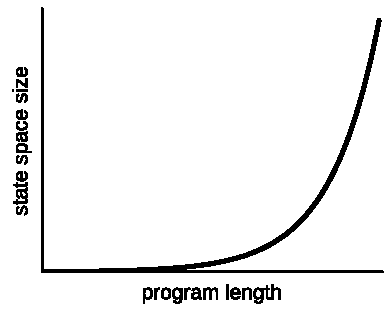
\includegraphics[width=0.4\textwidth]{exponence.pdf}
	\end{center}
\end{frame}

% better: remember to say, "If you're wondering what the deal is with "stateless"...
% the name is a historical accident & we can talk abt that in the Q+As"
\begin{frame}{Stateless Model Checking - The State Space}
	\begin{center}
		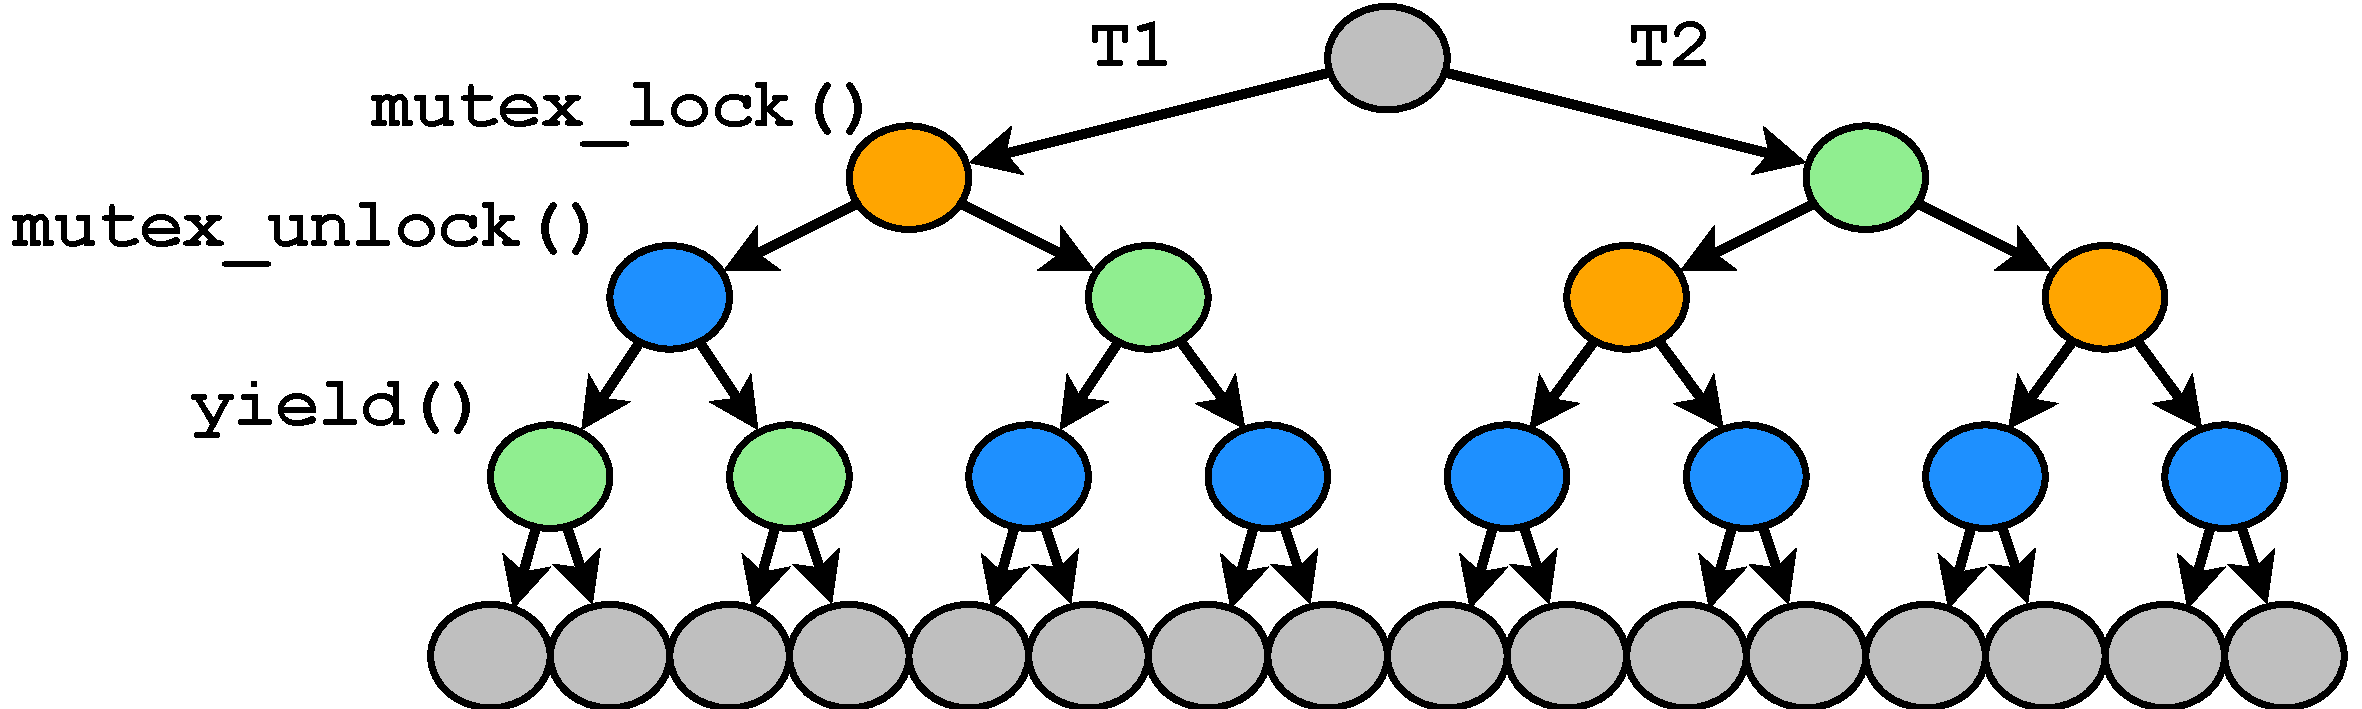
\includegraphics[width=0.96\textwidth]{../../oopsla/tree-maximal-only.pdf}
	\end{center}
	\linegap

	Possible interleavings (under given test case) represented as a tree
	\begin{itemize}
		\item Node: Intermediate execution state
		\item Edge: State transition from executing a thread
	\end{itemize}
	\linegap

	State space size depends on which {\bf preemption points} are used.
\end{frame}

\begin{frame}{Challenges} %\& Existing Coping Techniques}
	Unpredictable state space explosion
	\begin{itemize}
		%\item Equivalence reductions: DPOR {\em [Flanagan '05]}, MCR {\em [Huang '15]}
		\item Dynamic Partial Order Reduction (DPOR) {\em [Flanagan '05]}
			\begin{itemize}
				\item identifies \& skips equivalent interleavings
			\end{itemize}
		%\item Heuristic search ordering: ICB {\em [Musuvathi '08]}, PCT {\em [Burckhardt '10]}
		\item Iterative Context Bounding (ICB) {\em [Musuvathi '08]}
			\begin{itemize}
				\item finds bugs faster by prioritizing interleavings with fewer preemptions
			\end{itemize}
			\pause
		\item There will always be a {\bf bigger test case}...
	\end{itemize}
	\pause
	\linegap

	Too much manual intervention %for non-expert use
	\begin{itemize}
		\item State space size estimation {\em [Simsa '12]}
			% TODO: i just switched the order of these; see how that feels
		\item Manual kernel annotations {\em [Blum '12]} %{\tiny that's me!}
			\pause
		\item Widespread adoption requires {\bf fully automated instrumentation}...
	\end{itemize}
	\pause
	\linegap

	Sources of nondeterminism
	\begin{itemize}
		\item Timer-driven schedule nondeterminism (all prior work)
		\item Weak memory {\em [Zhang '15]},
			event-driven {\em [Jensen '15]}
			\pause
		\item {\bf Hardware transactional memory}...
	\end{itemize}
\end{frame}

%\begin{frame}{overview of state of art}
%	\begin{itemize}
%		\item so like, you got all this threads, right?
%		\item n then you just make em go any which way
%		\item see what all bugs come out
%	\end{itemize}
%\end{frame}

\begin{frame}{Thesis Statement}
	% data race pps (as well as txn equivalence)
	Combining %both
	theoretically-founded automatic reduction techniques
	% iterative deepening
	% (say smth like: "landslide also has a wealth of other user-tunable heuristics
	% for expert users, which you can read about in the document; for this talk i will focus just on the CPU budget thing")
	% XXX: need to prepare for the question -- "what evidence do you have that users actually want this cpu budget stuff",
	% ",or, that it helps vs just running something unlimited vs a normal icb test"
	% (well, for the 2nd half of the Q, i can talk about how ID outperforms ICB on verficiations)
	and user-informed heuristic ones,
	stateless model checking can sufficiently mitigate exponential explosion to be
	% education
	practical for inexperienced users
	%a practical testing technique for inexperienced users
	% htm
	% TODO: this last part you just added for this talk; does the thesis version of the statmeent need to include too?
	and real-world programs alike.
\end{frame}

\begin{frame}{Thesis Statement}
	% data race pps (as well as txn equivalence)
	\hilight{gray}{Combining %both
	theoretically-founded automatic reduction techniques
	% iterative deepening
	% (say smth like: "landslide also has a wealth of other user-tunable heuristics
	% for expert users, which you can read about in the document; for this talk i will focus just on the CPU budget thing")
	% XXX: need to prepare for the question -- "what evidence do you have that users actually want this cpu budget stuff",
	% ",or, that it helps vs just running something unlimited vs a normal icb test"
	% (well, for the 2nd half of the Q, i can talk about how ID outperforms ICB on verficiations)
	and user-informed heuristic ones, stateless model checking...}
	\begin{itemize}
		\item \hilight{sect-quicksand}{...can sufficiently mitigate exponential explosion...}\xspace
		% education
		%\item ...to be a practical testing technique for inexperienced users...
		\item \hilight{sect-410}{...to be practical for inexperienced users...}\xspace
		% htm
		% TODO: this last part you just added for this talk; does the thesis version of the statmeent need to include too?
		\item \hilight{sect-htm}{...and real-world programs alike.}\xspace
	\end{itemize}
\end{frame}


\begin{frame}{Contributions}
	\hilight{sect-quicksand}{The Quicksand algorithm %combines theory and heuristics to
	practically debugs and verifies many exponential state spaces.}
	\vspace{4.54em}

	\hilight{sect-410}{Landslide's automatic instrumentation makes MC accessible to students.}
	\vspace{4.54em}

	\hilight{sect-htm}{New reduction techniques for transactional memory keep MC up-to-date
	with the latest real-world concurrency techniques.}
	\vspace{4.54em}
\end{frame}
\begin{frame}{Outline}
	\hilight{sect-pastel-quicksand}{The Quicksand algorithm %combines theory and heuristics to
	practically debugs and verifies many exponential state spaces.} \\
	%\hilight{gray}{The Quicksandalgorithm makes MC appropriate for both educational and real-world programs.} \\
	\begin{itemize}
		\item {\bf Quicksand}
		\begin{itemize}
			\item Data-race preemption points \& algorithm overview
			\item Verification \& experimental results
		\end{itemize}
	\end{itemize}
	\hilight{sect-pastel-410}{Landslide's automatic instrumentation makes MC accessible to students.} \\
	%\hilight{gray}{Ad-hoc synchronization heuristics make MC accessible to student programmers.} \\
	\begin{itemize}
		\item {\bf Educational use}
		\begin{itemize}
			\item Pebbles \& Pintos OS projects
			\item Bug-finding, grades, \& surveys
		\end{itemize}
	\end{itemize}

	\hilight{sect-pastel-htm}{New reduction techniques for transactional memory keep MC up-to-date
	with the latest real-world concurrency techniques.} \\
	%\hilight{gray}{A new transactional concurrency model keeps MC applicable to the latest real-world techniques.} \\
	\begin{itemize}
		\item {\bf Transactional memory}
		\begin{itemize}
			\item Concurrency model \& failure injection
			\item Bug-finding \& verification
		\end{itemize}
	\end{itemize}
\end{frame}

%\begin{frame}{Outline}
%	guess i should outline my talk huh
%\end{frame}


%%%%%%%%%%%%%%%%%%%%%%%%%%%%%%%%%%%%%%%%%%%%%%%%%%%%%%%%%%%%%%%%%%%%%%%%%%%%%%%%
%%%%%%%%%%%%%%%%%%%%%%%%%%%%%%%%%%%%%%%%%%%%%%%%%%%%%%%%%%%%%%%%%%%%%%%%%%%%%%%%
%%%%%%%%%%%%%%%%%%%%%%%%%%%%%%%%%%%%%%%%%%%%%%%%%%%%%%%%%%%%%%%%%%%%%%%%%%%%%%%%

\section{Part 1}
\subsection{Quicksand}

\breakslide{\Large \bf \hilight{sect-quicksand}{Quicksand}}

\begin{frame}{Preemption Points}
	The burning question: ``Which {\bf preemption points} are important?''
	\linegap

	State space %of interleavings
	is {\em parameterized} by preemption points.
	\begin{itemize}
		\item Too few: Many bugs will go undetected
		\item Preempt everywhere: Completion is often infeasible % say: "for some programs"
	\end{itemize}
\end{frame}

\begin{frame}{Example (Revisited)}
	\begin{center}
	\begin{tabular}{ll}
		Initially \texttt{count = 0;} \\
		\\
		{\bf Thread 1} & {\bf Thread 2} \\
		\\
		\texttt{\hilight{darkorange}{mutex\_lock}(m);} \\
		\texttt{int tmp = count;} \\
								& \texttt{atomic\_xadd(\&count, 1);} \\
								& \texttt{\hilight{olivegreen}{yield}();} \\
								& \texttt{atomic\_xadd(\&count, 1);} \\
		\texttt{count = tmp + 1;} \\
								& \texttt{\hilight{pinkish}{assert(count >= 2);}} \\
		\texttt{\hilight{darkblue}{mutex\_unlock}(m);} \\
		\texttt{assert(count >= 1);}
	\end{tabular}
	\end{center}
\end{frame}

\begin{frame}{State Space (Revisited)}
	\begin{center}
		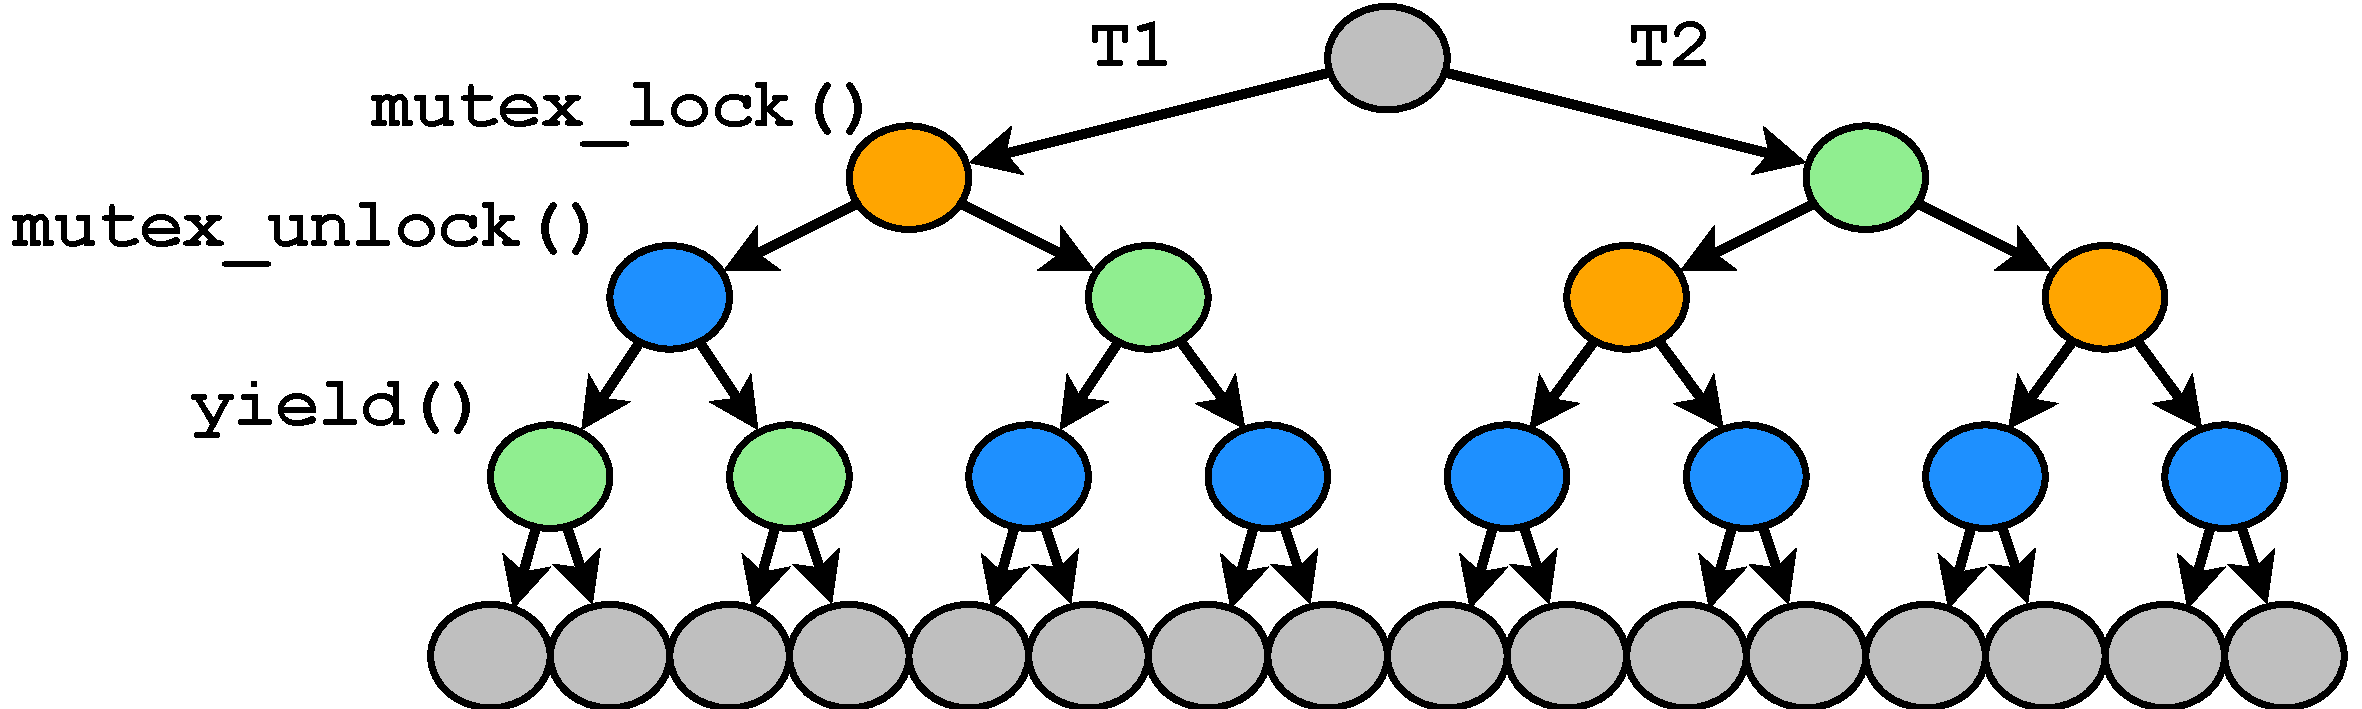
\includegraphics[width=0.96\textwidth]{../../oopsla/tree-maximal-only.pdf}
	\end{center}
	\linegap

	None of these branches contain the necessary preemption!
	\linegap

	A {\bf data-race preemption point} is required to find the bug.
\end{frame}

\begin{frame}{Data Race Analysis}
	A {\bf data race} is a pair of memory accesses between two threads, where:
	\begin{itemize}
		\item At least one of the accesses is a write
		\item The threads are not holding the same mutex
		\item Neither access {\em happens-before} the other
			%(e.g., no \texttt{cond\_signal()} in between)
			(e.g., no \texttt{cond\_wait()})
	\end{itemize}
	\pause
	\linegap

	%Prior model checkers hard-code a fixed set of PPs, committing to one state space in advance.
	%Prior model checkers commit to a fixed set of PPs in advance.
	Prior model checkers commit to fixed preemption points in advance.
	\begin{itemize}
		\item ``Preempt on {\tt mutex\_lock()}, {\tt mutex\_unlock()} only''
		\item ``Preempt on every single memory access''
	\end{itemize}
	\linegap

	Insight: Decide where to preempt on-the-fly
	% say: "...then attempt to cope with the resulting exponentially sized problem, however big it may be"

	%Two flavors
	%\begin{itemize}
	%	\item {\bf Pure HB}: Whether accesses were {\em observed simultaneously}, false-negative prone
	%		{\em [Lamport '78]}
	%	\item {\bf Limited HB}: Whether threads {\em could be reordered}, false-positive prone
	%		{\em [O'Callahan '03]}
	%\end{itemize}
\end{frame}

\begin{frame}{Quicksand (in Pictures)}
	\begin{center}
	\vspace{-0.88em}
	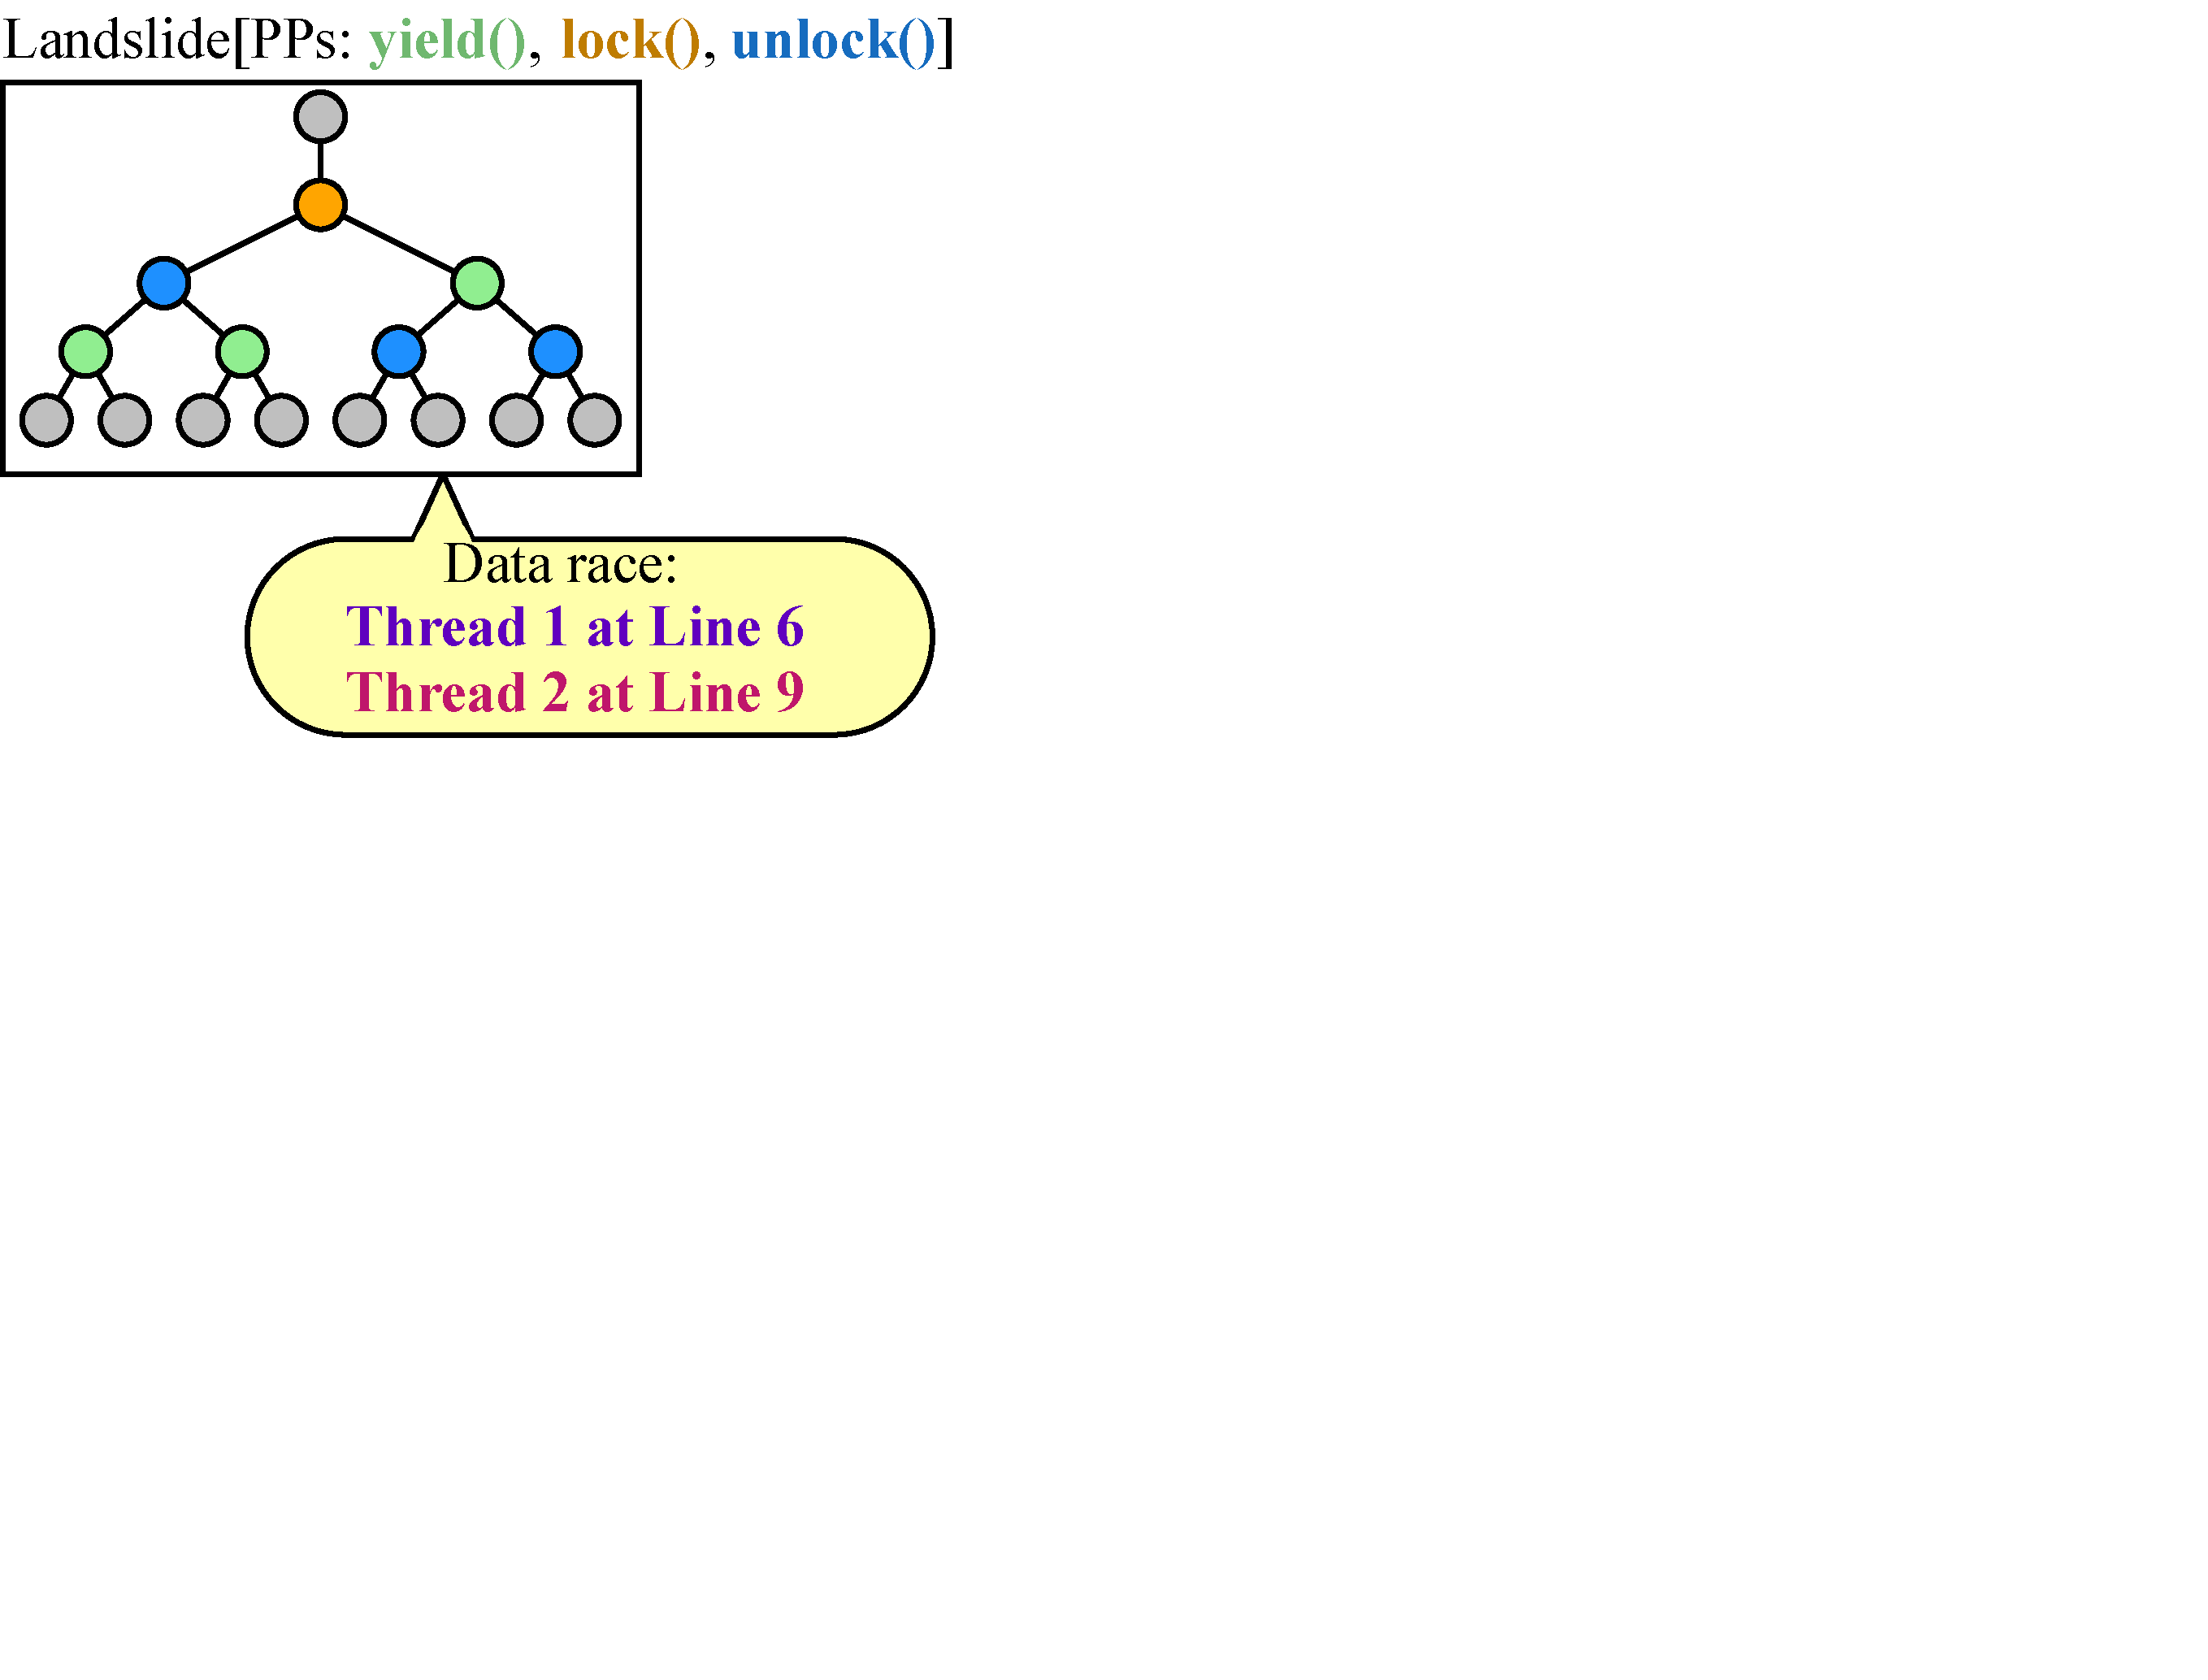
\includegraphics[width=0.86\textwidth]{../../oopsla/dr-jobs-1.pdf}
	\end{center}
\end{frame}
\begin{frame}{Quicksand (in Pictures)}
	\begin{center}
	\vspace{-0.88em}
	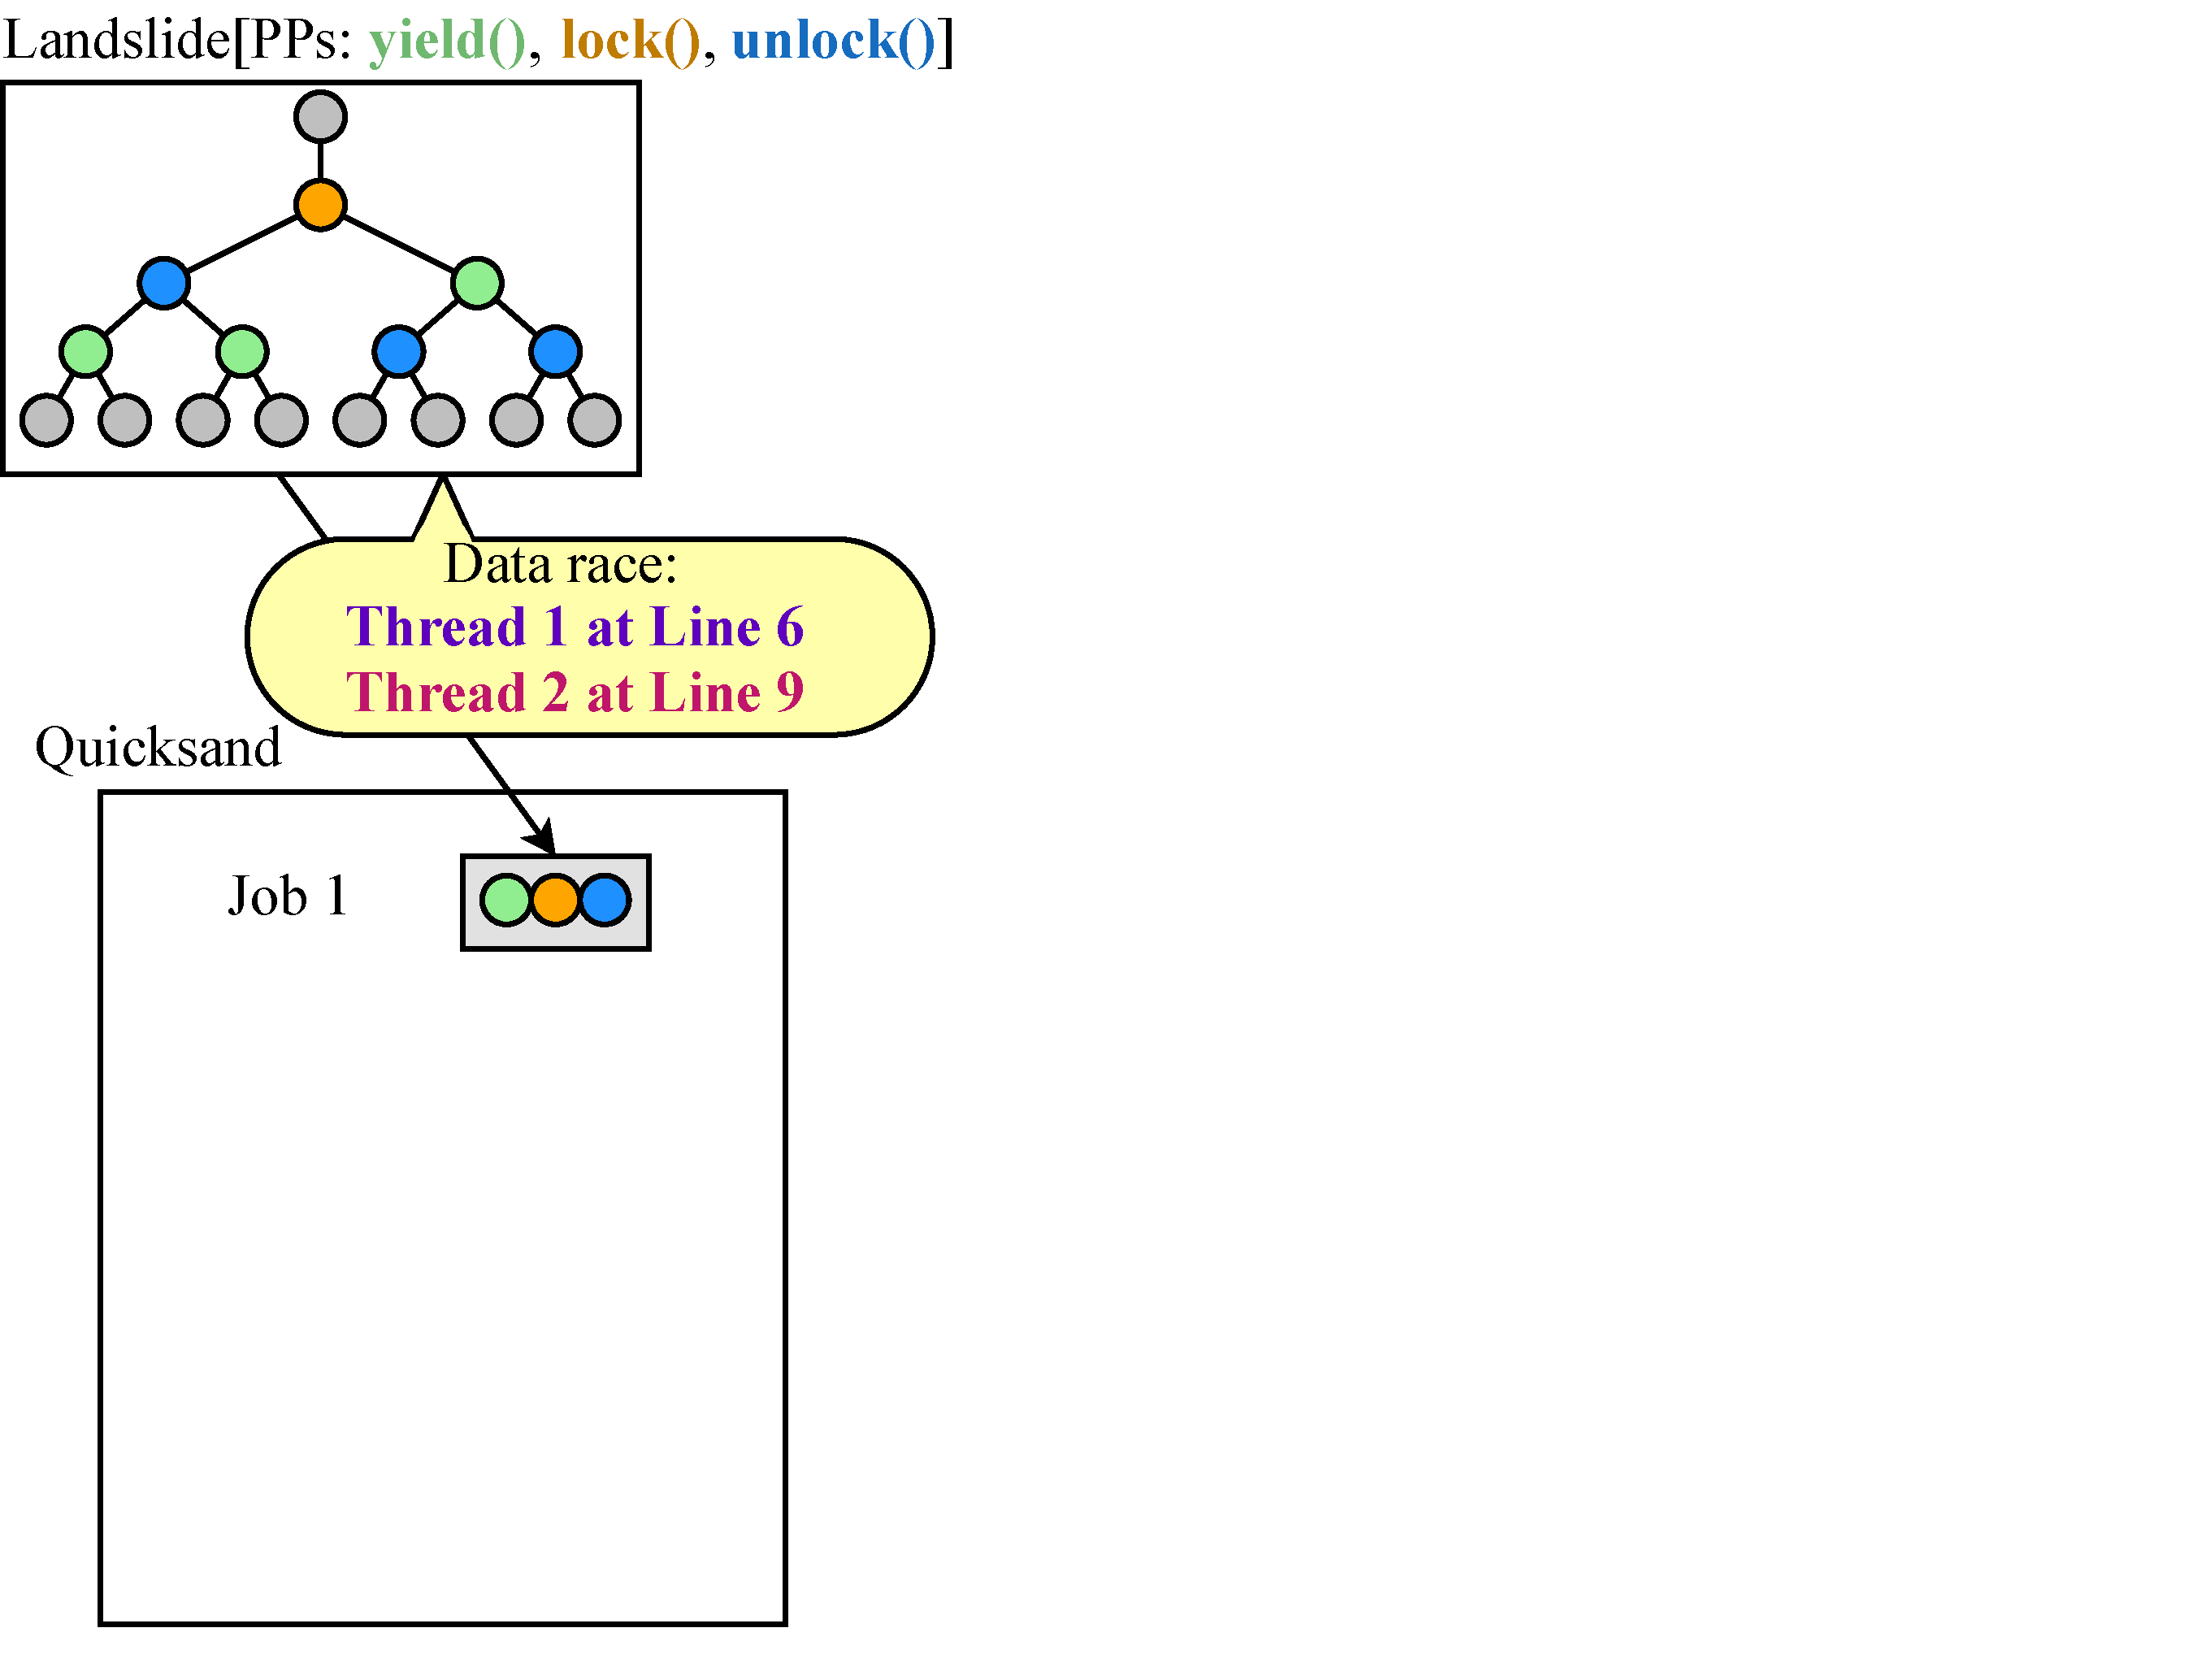
\includegraphics[width=0.86\textwidth]{../../oopsla/dr-jobs-2.pdf}
	\end{center}
\end{frame}
\begin{frame}{Quicksand (in Pictures)}
	\begin{center}
	\vspace{-0.88em}
	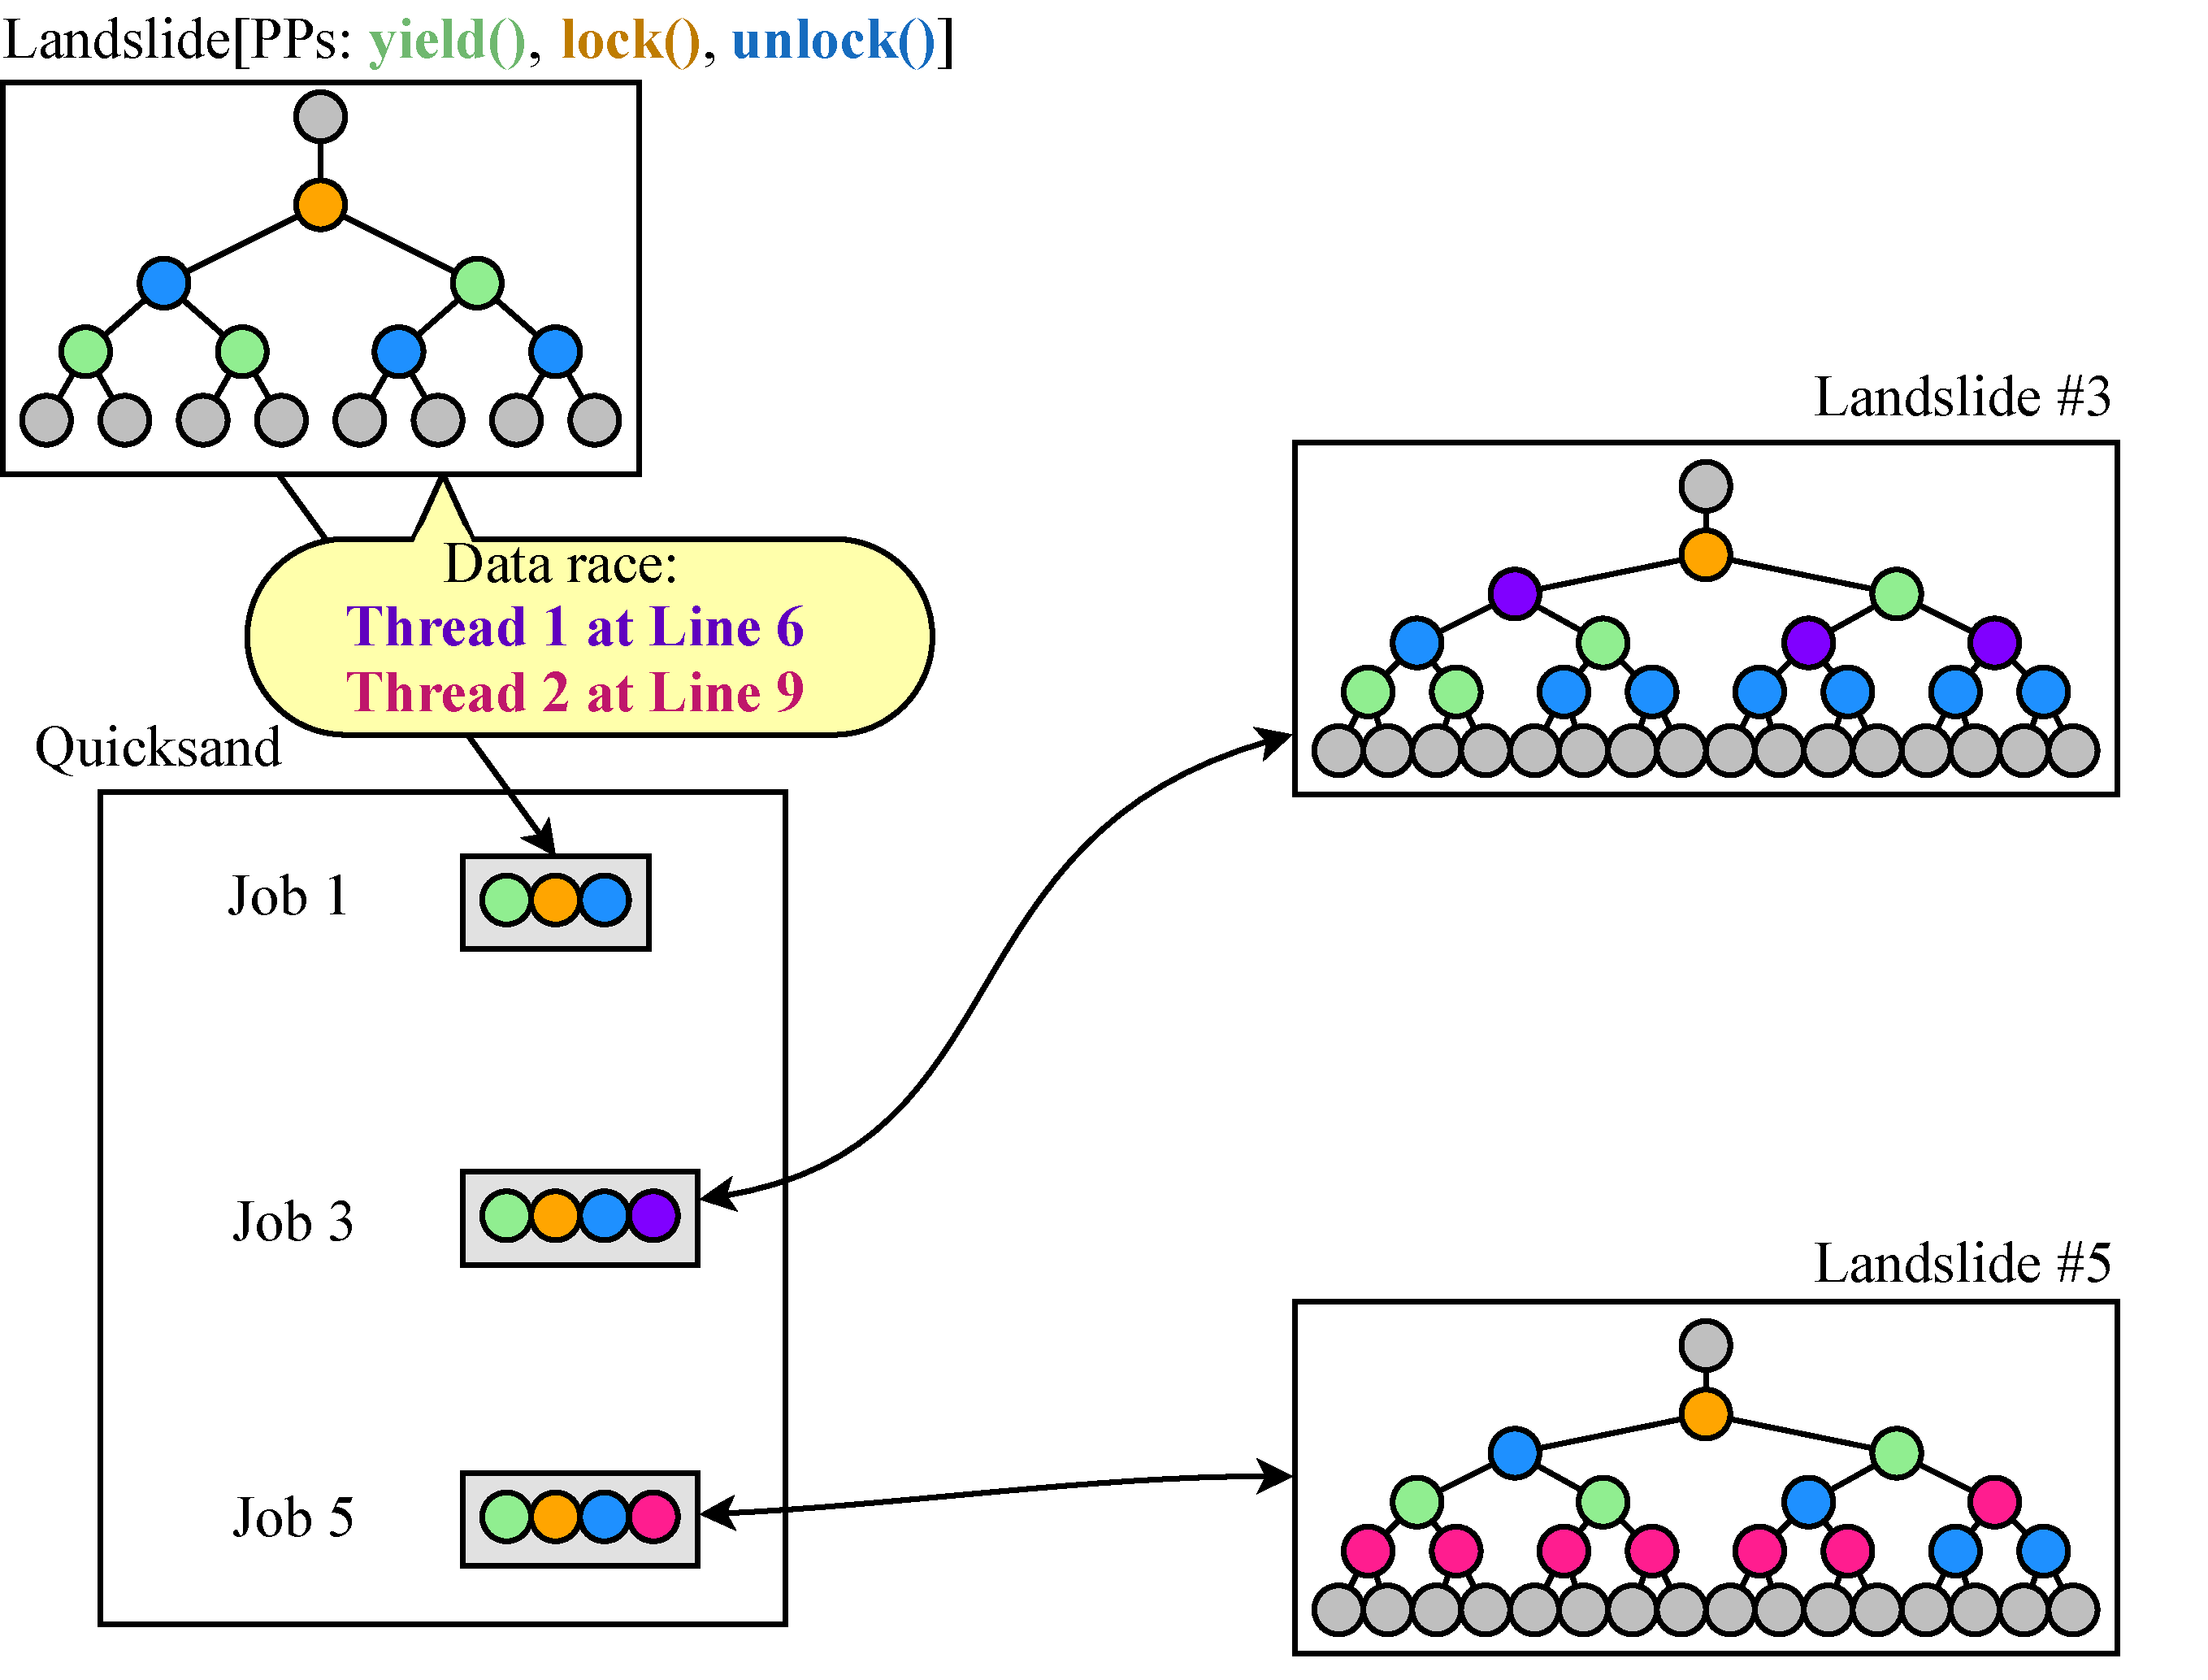
\includegraphics[width=0.86\textwidth]{../../oopsla/dr-jobs-3.pdf}
	\end{center}
\end{frame}
\begin{frame}{Quicksand (in Pictures)}
	\begin{center}
	\vspace{-0.88em}
	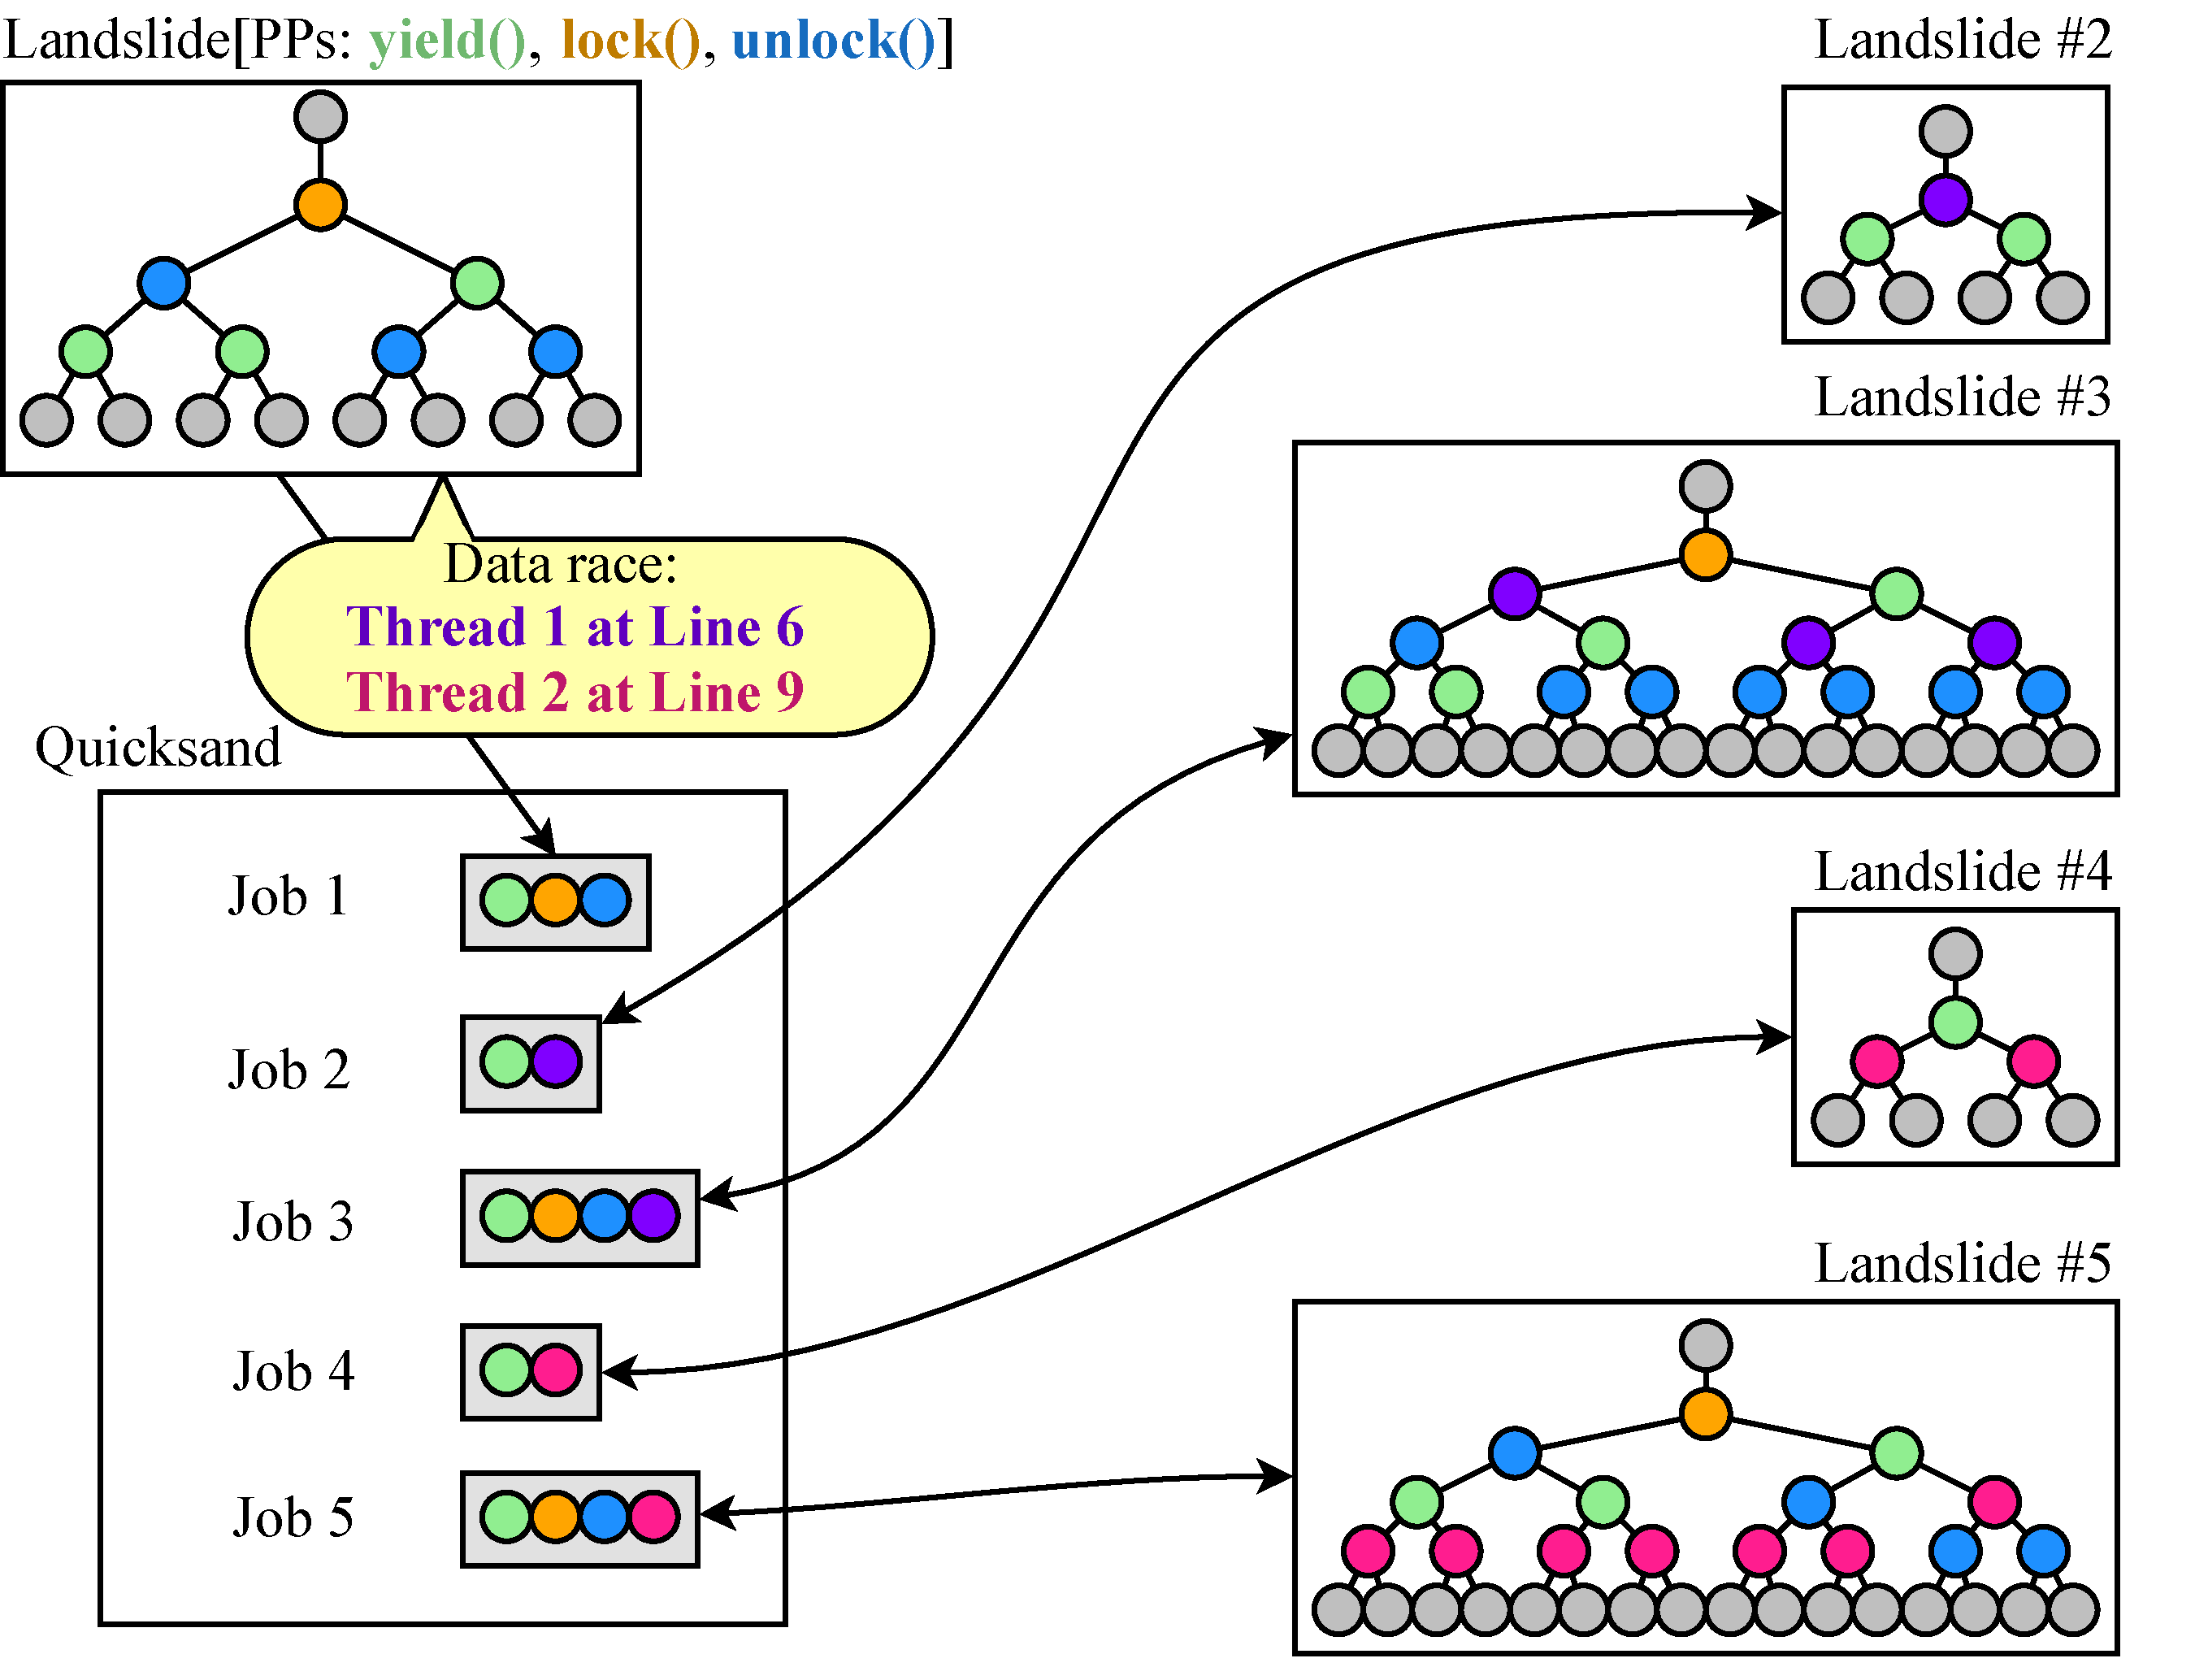
\includegraphics[width=0.86\textwidth]{../../oopsla/dr-jobs-4.pdf}
	\end{center}
\end{frame}
\begin{frame}{Quicksand (in Pictures)}
	\begin{center}
	\vspace{-0.88em}
	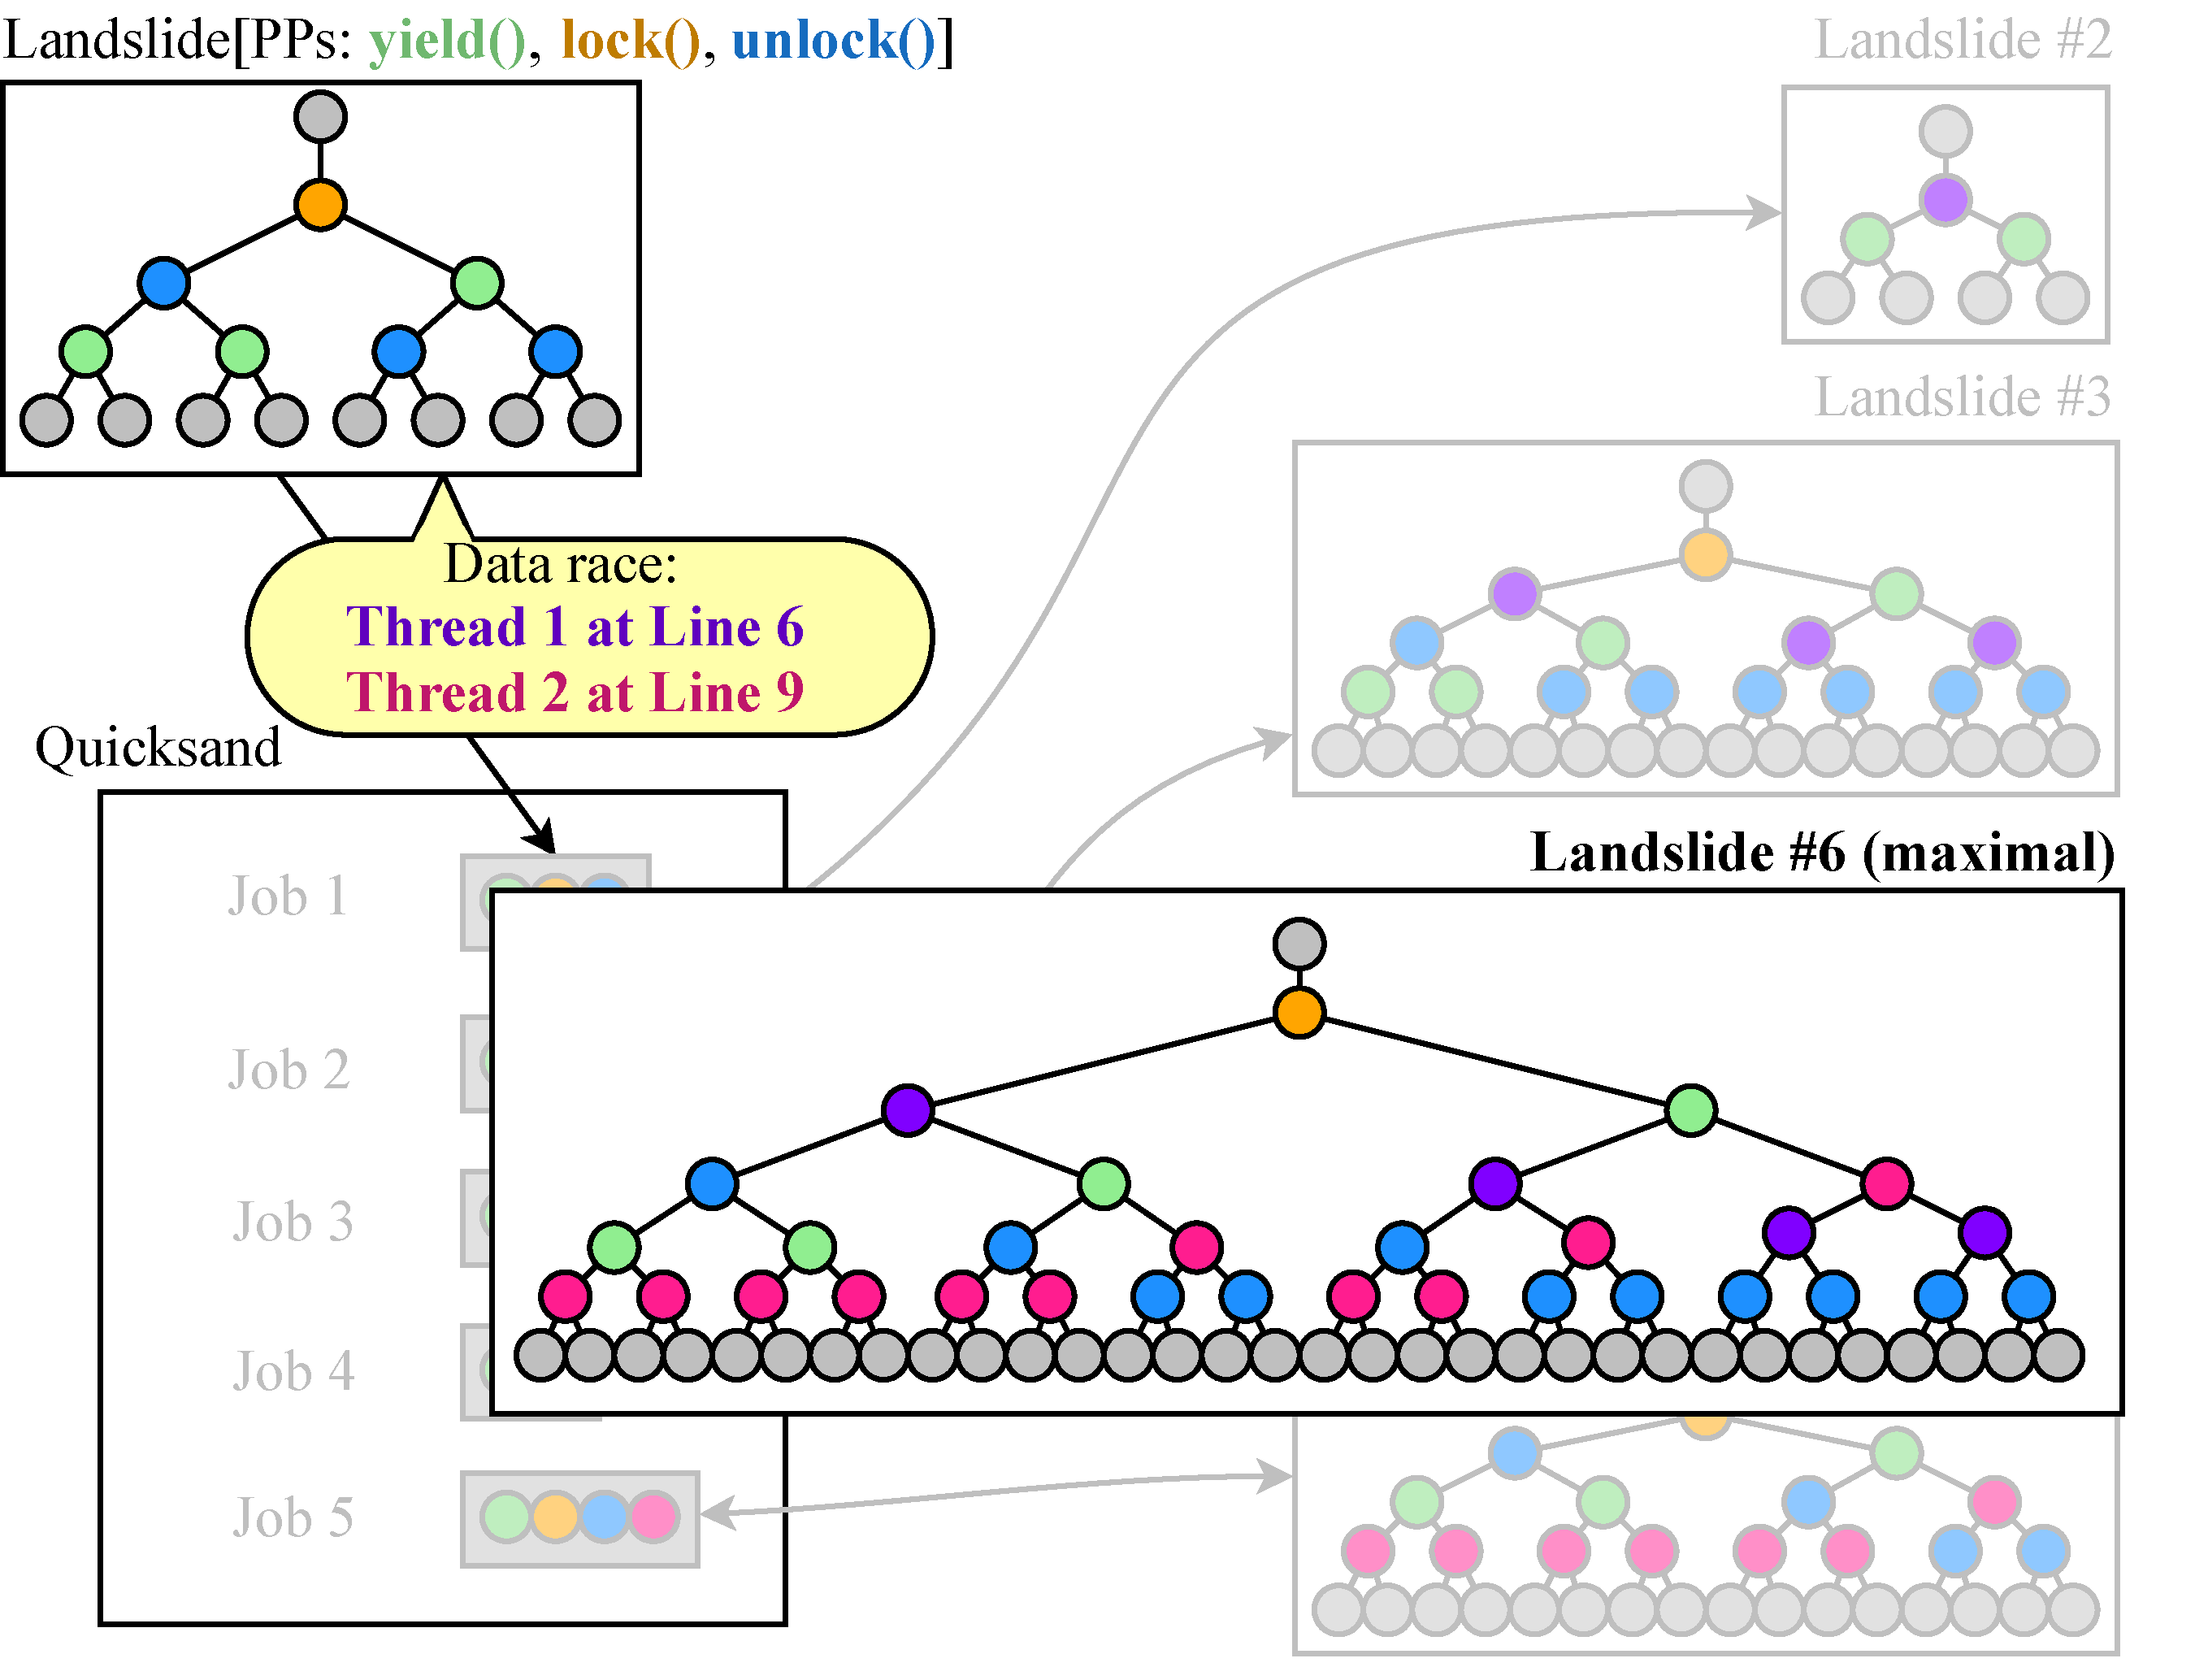
\includegraphics[width=0.86\textwidth]{dr-jobs-maximal.pdf}
	\end{center}
\end{frame}

% TODO put a pict of mario-man, i.e maximal state space

\begin{frame}{Total Verification}
	\textbf{Convergence theorem:} Testing maximal state space, after detecting all data races, $\equiv$ preempting everywhere!
	\begin{itemize}
		\item $\forall$ arbitrary buggy interleaving, $\exists$ equivalent interleaving % say 'under DPOR' i guess?
			using only sync/data-race PPs, \& Quicksand will eventually reach it.
			\begin{itemize}
				\item ({\em equivalence} defined under DPOR {\em [Flanagan '05]})
			\end{itemize}
	\end{itemize}
	\linegap

	Hence, Quicksand provides ``best of both worlds'':
	\begin{itemize}
		\item Provides total safety guarantee for small tests
		\item Finds bugs quickly for large tests when completion is infeasible
	\end{itemize}
\end{frame}

\begin{frame}{Evaluation}
	79 ``P2'' thread libraries from CMU, 78 ``Pintos'' kernels from U. Chicago \& Stanford
	\linegap

	%629 pairs of \{P2 or Pintos\} + test case
	629 pairs of P2 or Pintos + test case
	\linegap

	Each tested for 10 CPU-hours with
	\begin{itemize}
		\item Quicksand % parallelized 10-fold
			%, finding data-race candidates with...
			%\begin{itemize}
			%	\item ...``Pure'' Happens-Before analysis {\em [Lamport '78]}
			%	\item ...``Limited'' Happens-Before analysis {\em [O'Callahan '03]}
			%\end{itemize}
		\item Stand-alone Landslide using ICB {\em [Musuvathi '08]}, preempting at...
			\begin{itemize}
				\item ...synchronization APIs only {\em [Simsa '10]}
				\item ...all shared memory accesses
					%{\em [Holzmann '97]} % not spin
					{\em [Yang '08]} % inspect
			\end{itemize}
	\end{itemize}
\end{frame}

\begin{frame}{Results - Bugs found (CPU time)}
	\begin{center}
		\includegraphics[width=0.8\textwidth]{../quicksand-bugs-talkver.pdf}
	\end{center}
\end{frame}
\begin{frame}{Results - Bugs found (wall-clock time)}
	\begin{center}
		\includegraphics[width=0.8\textwidth]{../quicksand-bugs-wallclock-talkver.pdf}
	\end{center}
\end{frame}
\begin{frame}{Results - Full verifications}
	\begin{center}
		\includegraphics[width=0.8\textwidth]{../quicksand-verifs-talkver.pdf}
	\end{center}
\end{frame}

\begin{frame}{Summary}
	Use data-race analysis to add new preemption points in a feedback loop
	\linegap

	Enough time to saturate \& test every data-race? Full verification
	\linegap

	Otherwise? Quicksand's heuristic search ordering finds bugs faster anyway
	%\pause
	%\linegap

	%Future work
	%\begin{itemize}
	%	\item Extend proof to weak memory
	%	\item Incorporate ICB in Quicksand
	%	\item Improve estimation accuracy
	%\end{itemize}
\end{frame}

%%%%%%%%%%%%%%%%%%%%%%%%%%%%%%%%%%%%%%%%%%%%%%%%%%%%%%%%%%%%%%%%%%%%%%%%%%%%%%%%
%%%%%%%%%%%%%%%%%%%%%%%%%%%%%%%%%%%%%%%%%%%%%%%%%%%%%%%%%%%%%%%%%%%%%%%%%%%%%%%%
%%%%%%%%%%%%%%%%%%%%%%%%%%%%%%%%%%%%%%%%%%%%%%%%%%%%%%%%%%%%%%%%%%%%%%%%%%%%%%%%

\section{Part 2}
\subsection{Education}

\breakslide{\Large \bf \hilight{sect-410}{Education}}

\begin{frame}{Setting}
	%CMU (15-410, S'15-S'18), PSU (CMPSC 473, S'18)
	CMU (15-410), PSU (CMPSC 473)
	\begin{itemize}
		\item Thread library (``P2'')
			\begin{itemize}
				\item POSIX-like userspace thread library %(also teams of 2)
				\item Reference ``Pebbles'' kernel provided
					% say: later they implement this in p3
				\item Fixed APIs $\rightarrow$ instrumentation can be automated
				\item Still needs heuristics to handle ad-hoc synchronization
			\end{itemize}
			% FIXME: need introduce p3 here?
			% Or cut?
		\item Kernel (``P3'') - reimplement said reference kernel (CMU only)
	\end{itemize}
	\pause
	\linegap

	%U. Chicago (CMSC 23000, F'17)
	U. Chicago (CMSC 23000)
	\begin{itemize}
		\item Pintos %(``threads'' and ``userprog'')
		\begin{itemize}
			\item Basecode provides round-robin scheduler, synchronization, VM, loader
			\item ``threads'': Students implement priority scheduling, sleep
		%\end{itemize}
		%\linegap

		%\item Processes (``userprog'')
		%\begin{itemize}
				% fork is part of exec and the loader is already provided
			\item ``userprog'': UNIX-like process lifecycle
				({\tt exec}, % students don't really implement any complciated part of this though
				% i think just like. the argument copying??
				{\tt exit}, {\tt wait})
			%\item File descriptor management ({\tt create}, {\tt remove}, {\tt open}, {\tt read}, ...)
				% filesys project is beyond scope of landslide
				% DONT say: the u chicago professor chose to discard the hard concurrency parts
				% DO say, if pressured: device driver concurrency would require more engineering,
				% so we chose to limit it to these two projex
		\end{itemize}
	\end{itemize}
\end{frame}

\begin{frame}{Instrumentation}
	Understanding concurrency primitives/APIs
	\begin{itemize}
		\item Kernel-level testing requires manual annotation {\em [Blum '12]}
		\item P2 (fixed APIs), Pintos (basecode provided) annotated automatically
	\end{itemize}
	\pause
	\linegap

	Ad-hoc synchronization (e.g. {\tt while (!ready) yield();})
	\begin{itemize}
		\item Not an infinite loop bug!
		\item Heuristically ``block'' threads when 10+ {\tt yield()}s %({\tt xchg}, etc.)
		\item Existing memory analysis %(DPOR)
			on loop condition to unblock
			\begin{itemize}
					% TODO: cut this and just say it out loud?
				\item (e.g., what other thread writes to {\tt ready}?)
				% it's kinda... idk how to critique its unsoundness.
				% they self-admit to the unsoundness but like, leaving the cycle in,
				% is the wrong approach to begin with
					% TODO: move this to bonus slides, save a min of expl
				%\item Prior work {\em [Coons '13]} likely to leave threads blocked too long
			\end{itemize}
			\pause
		\item ``Ok, what if I just {\tt yield()} 10 times because I feel like it?''
			\begin{itemize}
				\item If deadlock suspected, try waking up to avoid false positives
			\end{itemize}
		%\item Check for false-positive blocking to avoid false-positive deadlocks
	\end{itemize}


	% Unlike kernels [Blum '12], P2 can be......
	% TODO talk abt yield loops, 
	% compare to prior technique - delay abounding - which sucks bc (verify this by reading BPOR) it doesn't actually
	% wake up the other thread at the right time (using memory conflix)

	% pintos - bunch of gross patch stuff lmao
\end{frame}

% do even need this slide?
%\begin{frame}{Evaluation Questions}
%	asfda % TODO
%	% submit better projects?
%	% get better grades?
%	% like the experience?
%\end{frame}

\begin{frame}{Method}
	P2 (CMU + PSU)
	\begin{itemize}
		\item Guest lecture midway during project
		\item Landslide (+ Quicksand) provided to students with 6 test cases %and user guide
		\item Recorded code snapshots and bugs found each use (CMU only)
		\item Surveyed students on usability, false positives, etc.
	\end{itemize}
	\pause
	\linegap

	Pintos (U. Chicago)
	\begin{itemize}
		\item TA %(Kevin Zhao)
			ran Landslide on {\em threads} and {\em userprog} submissions
		\item Returned preemption traces to students after deadline
		\item Surveyed students on ease of debugging, etc.
	\end{itemize}
	% TODO: irb stuff in a bonus slide
\end{frame}

\begin{frame}{Results}
	Participation
	\begin{itemize}
		\item CMU: 103/177 students (7 semesters)
		\item U. Chicago: 4/21 students (1 semester)
		\item PSU: 38/136 students (1 semester)
	\end{itemize}
	\linegap

	Bug-finding
	\begin{itemize}
		\item CMU: 115 deterministic, 122 concurrency bugs in 75/103 P2s
		\item U. Chicago: 3 deterministic, 4 concurrency bugs in 3/4 kernels
			% TODO: what to do abt this bullet pts
			%\pause
		\item PSU: (no log collection) %due to IRB issues)
		% \item Case study tej
	\end{itemize}
\end{frame}

\begin{frame}{Effect on Grades (CMU)}
	Compared Landslide users' vs. non-users' submitted P2 grades...
	\begin{itemize}
		\item ``Does Landslide help students submit better projects?''
	\end{itemize}
	\linegap

	%...as well as subsequent P3 (kernel) grades
	...as well as subsequent kernel grades
	\begin{itemize}
		\item ``Does Landslide teach students lasting lessons about concurrency?''
	\end{itemize}
\end{frame}

\begin{frame}{Effect on Grades (CMU)}
	\begin{center}
		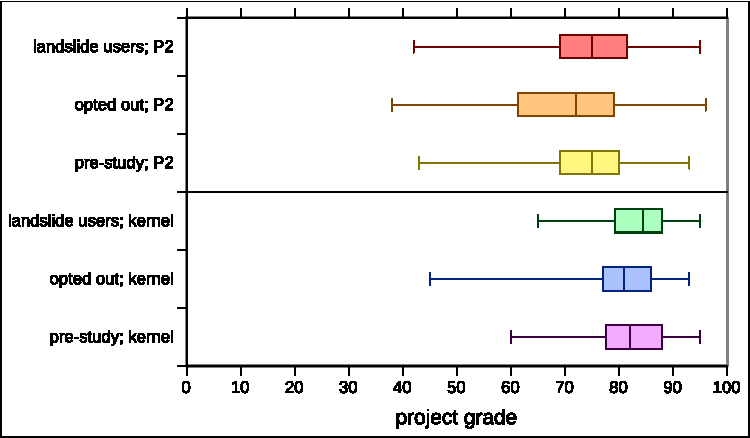
\includegraphics[width=\textwidth]{../photo-of-ze-studence.pdf}
	\end{center}
\end{frame}

% TODO: put p values
\begin{frame}{Effect on Grades (CMU)} % - statistically significant?}
	\begin{center}
		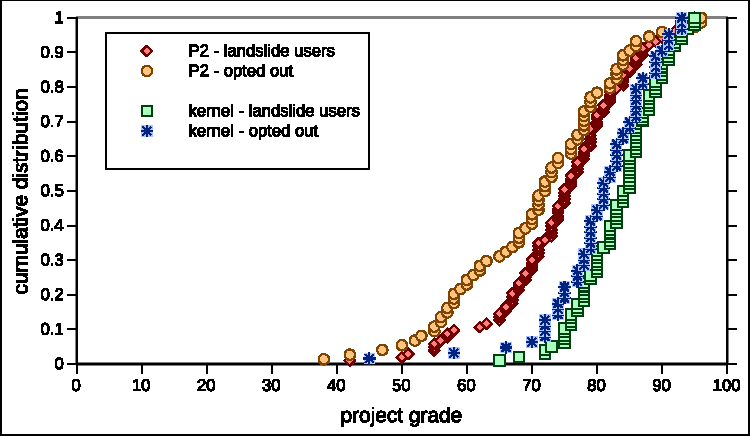
\includegraphics[width=\textwidth]{photo-of-ze-studence-cdf-no-pre-study.pdf}
	\end{center}
\end{frame}

\begin{frame}{Effect on Grades (CMU)} % - statistically significant?}
	\begin{center}
		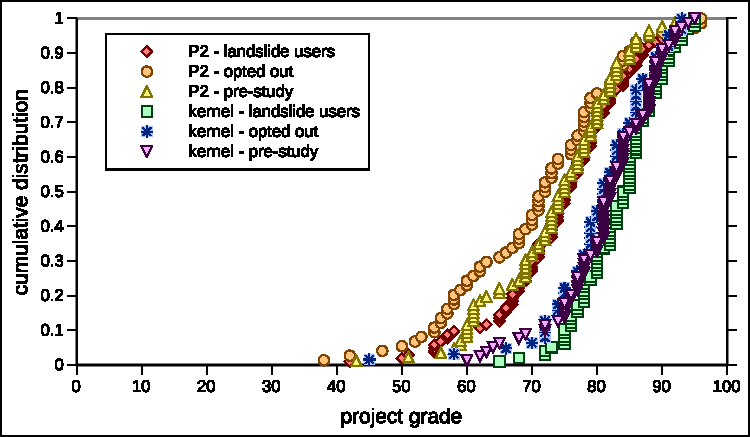
\includegraphics[width=\textwidth]{../photo-of-ze-studence-cdf.pdf}
	\end{center}
\end{frame}

%\begin{frame}{Statistical Significance}
%	Compared %users' vs. non-users'
%	grade distributions with k-sample Anderson-Darling {\em [A., D. '52]}
%	\linegap
%
%	Control 1: non-users from {\bf same semester}
%	\begin{itemize}
%		\item {\bf P2} grade distributions differ with $p = 0.036 < 0.05$
%		\item {\bf P3} grade distributions differ with $p = 0.034 < 0.05$
%			\pause
%		\item Possible bias: stronger students volunteer for Landslide in first place
%	\end{itemize}
%	\pause
%	\linegap
%
%	Control 2: non-users from {\bf past semesters} (when Landslide not offered)
%	\begin{itemize}
%		\item {\bf P2} grade distributions differ with $p = 0.671$...
%		\item {\bf P3} grade distributions differ with $p = 0.145$...
%			\pause
%		\item Possible bias: grading criteria may drift across semesters
%			% FIXME does this bullet belong in this sub list
%		\item Possible bias: maybe Landslide finds bugs the official tests don't
%	\end{itemize}
%\end{frame}

\begin{frame}{Survey}
	14(ish) questions, investigate both education \& happiness
	\begin{itemize}
		\item {\bf Education:} Did Landslide help students learn more from P2?
		\item {\bf Happiness:} Did Landslide help students save time/effort?
	\end{itemize}
	\pause
	\linegap

	Self-report any {\bf false positives}
	\begin{itemize}
		\item Landslide crashes aside, 3 FP bug reports, all simple bugs (now fixed)
			% nonexistent MAGIC_BREAK bc of different address space in shell
			% simultaneous landslides corrupt each other
			% invalid heap access when new_pages "too close"
		\item No FPs related to yield-loop/etc heuristics
	\end{itemize}
	\linegap

	Self-report opinions {\bf whether it was worthwhile}
	\begin{itemize}
		\item Mostly ``worked as advertised'' praise
		\item One PSU student found a bug from inspecting a data-race by hand,
			after Landslide timed out testing with no bug report
	\end{itemize}
\end{frame}

\begin{frame}{Survey Results} % (educational value)}
	\begin{center}
		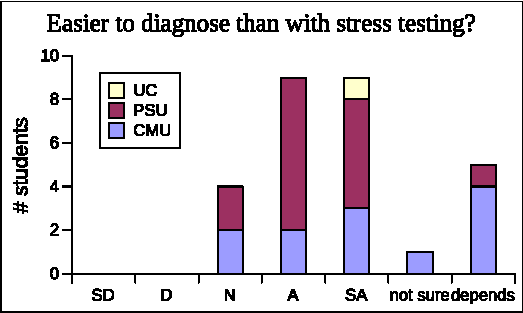
\includegraphics[width=\textwidth]{../survey6.pdf} % easier to diagnose?
	\end{center}
\end{frame}

%\begin{frame}{Survey Results} % (happiness value)}
%	\begin{center}
%		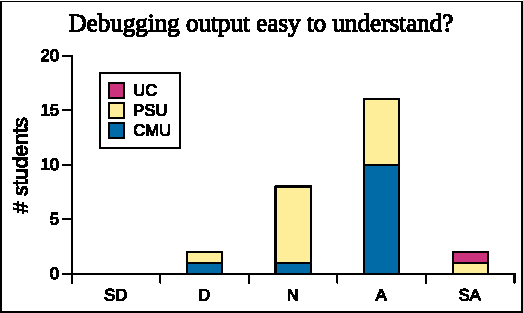
\includegraphics[width=\textwidth]{../survey5.pdf} % easy to understand?
%	\end{center}
%\end{frame}

\begin{frame}{Survey Results} % (educational value)}
	\begin{center}
		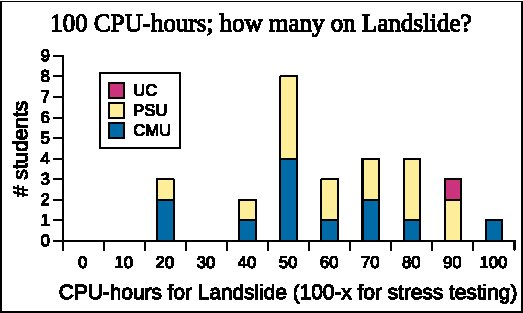
\includegraphics[width=\textwidth]{../survey9.pdf} % 100 cpu hours
	\end{center}
\end{frame}

\begin{frame}{Survey Results} % (educational value)}
	\begin{center}
		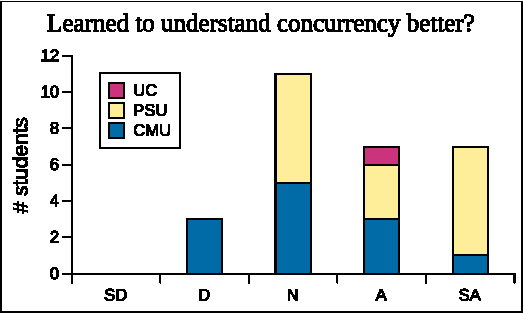
\includegraphics[width=\textwidth]{../survey8.pdf} % learned to understand concurrency
	\end{center}
\end{frame}

\begin{frame}{Survey Results} % (happiness value)}
	\begin{center}
		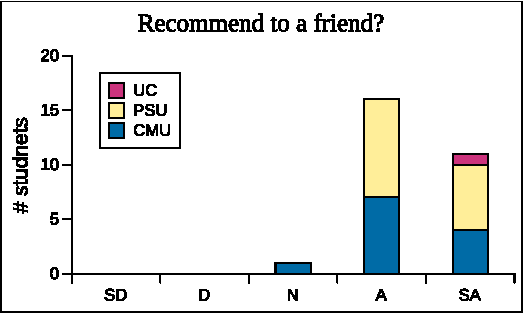
\includegraphics[width=\textwidth]{../survey10.pdf} % recommend to friend
	\end{center}
\end{frame}

\begin{frame}{Summary}
	Landslide helps students find \& fix bugs during projects
	% TODO: should this be moved ot the earlier bug finding slide
	\begin{itemize}
		\item 73\% of CMU users found $\ge 1$ bug
		\item 56\% of CMU users fixed $\ge 1$ bug
		\item 34\% of CMU users fixed all found bugs
	\end{itemize}
	\linegap

	Effect on overall project grades: ???
	\begin{itemize}
		\item Compensating for experimental bias difficult w/human subjects...
	\end{itemize}
	\linegap

	Survey results showed students ``enlightenedly happy'' % dave eckhardt scare quotes if i ever saw some
	\linegap

	15-410 course staff now including Landslide in official grading :)
\end{frame}


%%%%%%%%%%%%%%%%%%%%%%%%%%%%%%%%%%%%%%%%%%%%%%%%%%%%%%%%%%%%%%%%%%%%%%%%%%%%%%%%
%%%%%%%%%%%%%%%%%%%%%%%%%%%%%%%%%%%%%%%%%%%%%%%%%%%%%%%%%%%%%%%%%%%%%%%%%%%%%%%%
%%%%%%%%%%%%%%%%%%%%%%%%%%%%%%%%%%%%%%%%%%%%%%%%%%%%%%%%%%%%%%%%%%%%%%%%%%%%%%%%

\section{Part 3}
\subsection{Transactional Memory}
\newcommand\xbegin{\texttt{\_xbegin()}\xspace}
\newcommand\xend{\texttt{\_xend()}\xspace}
\newcommand\xabort{\texttt{\_xabort()}\xspace}

\breakslide{\Large \bf \hilight{sect-htm}{Transactional Memory}}

\begin{frame}{Example}
	\begin{center}
		\begin{tabular}{l}
			\texttt{if (\hilight{darkorange}{\_xbegin}() == SUCCESS) \{} \\ %\_XBEGIN\_STARTED) \{} \\
			%\texttt{} \\
			%\texttt{} \\
			\texttt{~~~~count++;} \\
			\texttt{~~~~\hilight{darkblue}{\_xend}();} \\
			\texttt{\} else \{}\\ %if (status != \_XABORT\_EXPLICIT) \{} \\
			\texttt{~~~~\hilight{darkorange}{mutex\_lock}(\&count\_lock);} \\
			\texttt{~~~~count++;} \\
			\texttt{~~~~\hilight{darkblue}{mutex\_unlock}(\&count\_lock);} \\
			\texttt{\}} \\
		\end{tabular}
	\end{center}
	% TODO: cite orig software TM, intel HTM
\end{frame}

\begin{frame}{HTM Execution Semantics}
	Attempting a transaction
	\begin{itemize}
		\item Code between \xbegin and \xend is provisionally executed
		\item All writes kept in CPU cache until \xend
		\item \xend commits changes atomically (w.r.t. other CPUs)
	\end{itemize}
	\pause
	\linegap

	Transaction failure
	\begin{itemize}
		\item Possible reasons:
			\begin{itemize}
				\item Memory conflict with another thread
				\item False sharing (conflict on same cache-line)
				\item Cache eviction, random interrupt, ...
			\end{itemize}
		\item Changes discarded, local state reverted, \xbegin returns failure
		\item {\tt else} branch runs some user-supplied backup plan
	\end{itemize}
\end{frame}

\begin{frame}{Model Checking Transactional Programs}
	What does it mean to MC a program?
	\begin{itemize}
		\item Capture all sites of nondeterminism as preemption points
		\item Control nondeterminism to force each possibility at each point
			\begin{itemize}
				\item (identifying equivalences to prune redundant branches)
			\end{itemize}
	\end{itemize}
	\pause
	\linegap

	MCing a transactional program
	\begin{itemize}
		\item Simulate TM, interleaving transactions, rolling-back upon conflicts
			\begin{itemize}
				\item slow; invites state space explosion
			\end{itemize}
		\item Enforce atomicity via scheduler, anticipate aborts on every transaction
			%via analysis
			%\begin{itemize}
			%	\item (under HTM, all transactions might abort)
			%\end{itemize}
		\item Suffices to enumerate all {\em observationally-equivalent} schedules.
	\end{itemize}
\end{frame}

\begin{frame}{Example}
	\begin{center}
		\begin{tabular}{l|l}
			{\bf Thread 1} & {\bf Thread 2} \\
			\hline
			{\tt \hilight{darkorange}{\_xbegin}() == SUCCESS} \\
			{\tt count++;} \\
				& {\tt \hilight{darkorange}{\_xbegin}() == SUCCESS} \\
				& {\tt count++;} \\
				& {\tt \hilight{darkblue}{\_xend}();} \\
			{\tt \hilight{darkblue}{\_xend}()}...? \\
			{\em <conflict detected>} \\
			\\
			{\tt \hilight{darkorange}{\_xbegin}() == ABORTED} \\
			{\tt \hilight{darkorange}{mutex\_lock}(...);} \\
			{\tt count++;} \\
			{\tt \hilight{darkblue}{mutex\_unlock}(...);} \\
		\end{tabular}
	\end{center}
\end{frame}

\begin{frame}{Concurrency model}
	What are a transactional program's {\em observable} behaviours?
	\begin{itemize}
		\item Transactional writes, if successful, appear atomically %to other threads
		\begin{itemize}
			\item Equivalent to a lock protecting that state
				% note that also inserting DR PPs within a transaction is not allowed
		\end{itemize}
			\pause
		\item Simultaneous transactions succeed only if no conflicts
		\begin{itemize}
			\item Equivalent
				%(modulo performance)
				to serialize independent transactions
		\end{itemize}
			\pause
		\item Failing transactions' effects rolled-back with no trace
		\begin{itemize}
			\item Treat each \xbegin as a failure injection point
		\end{itemize}
	\end{itemize}
	\pause
	\linegap

	Equivalence theorem
	\begin{itemize}
		\item Safe to automatically skip all interleavings within transactions %$\qed$
			\begin{itemize}
				\item Exponential state space reduction
				\item Traditional reduction (DPOR) applied on top
			\end{itemize}
		%\item More in bonus slides...
	\end{itemize}
\end{frame}

\begin{frame}{Failure Injection - 2 dimensions of concurrency}
	\begin{center}
		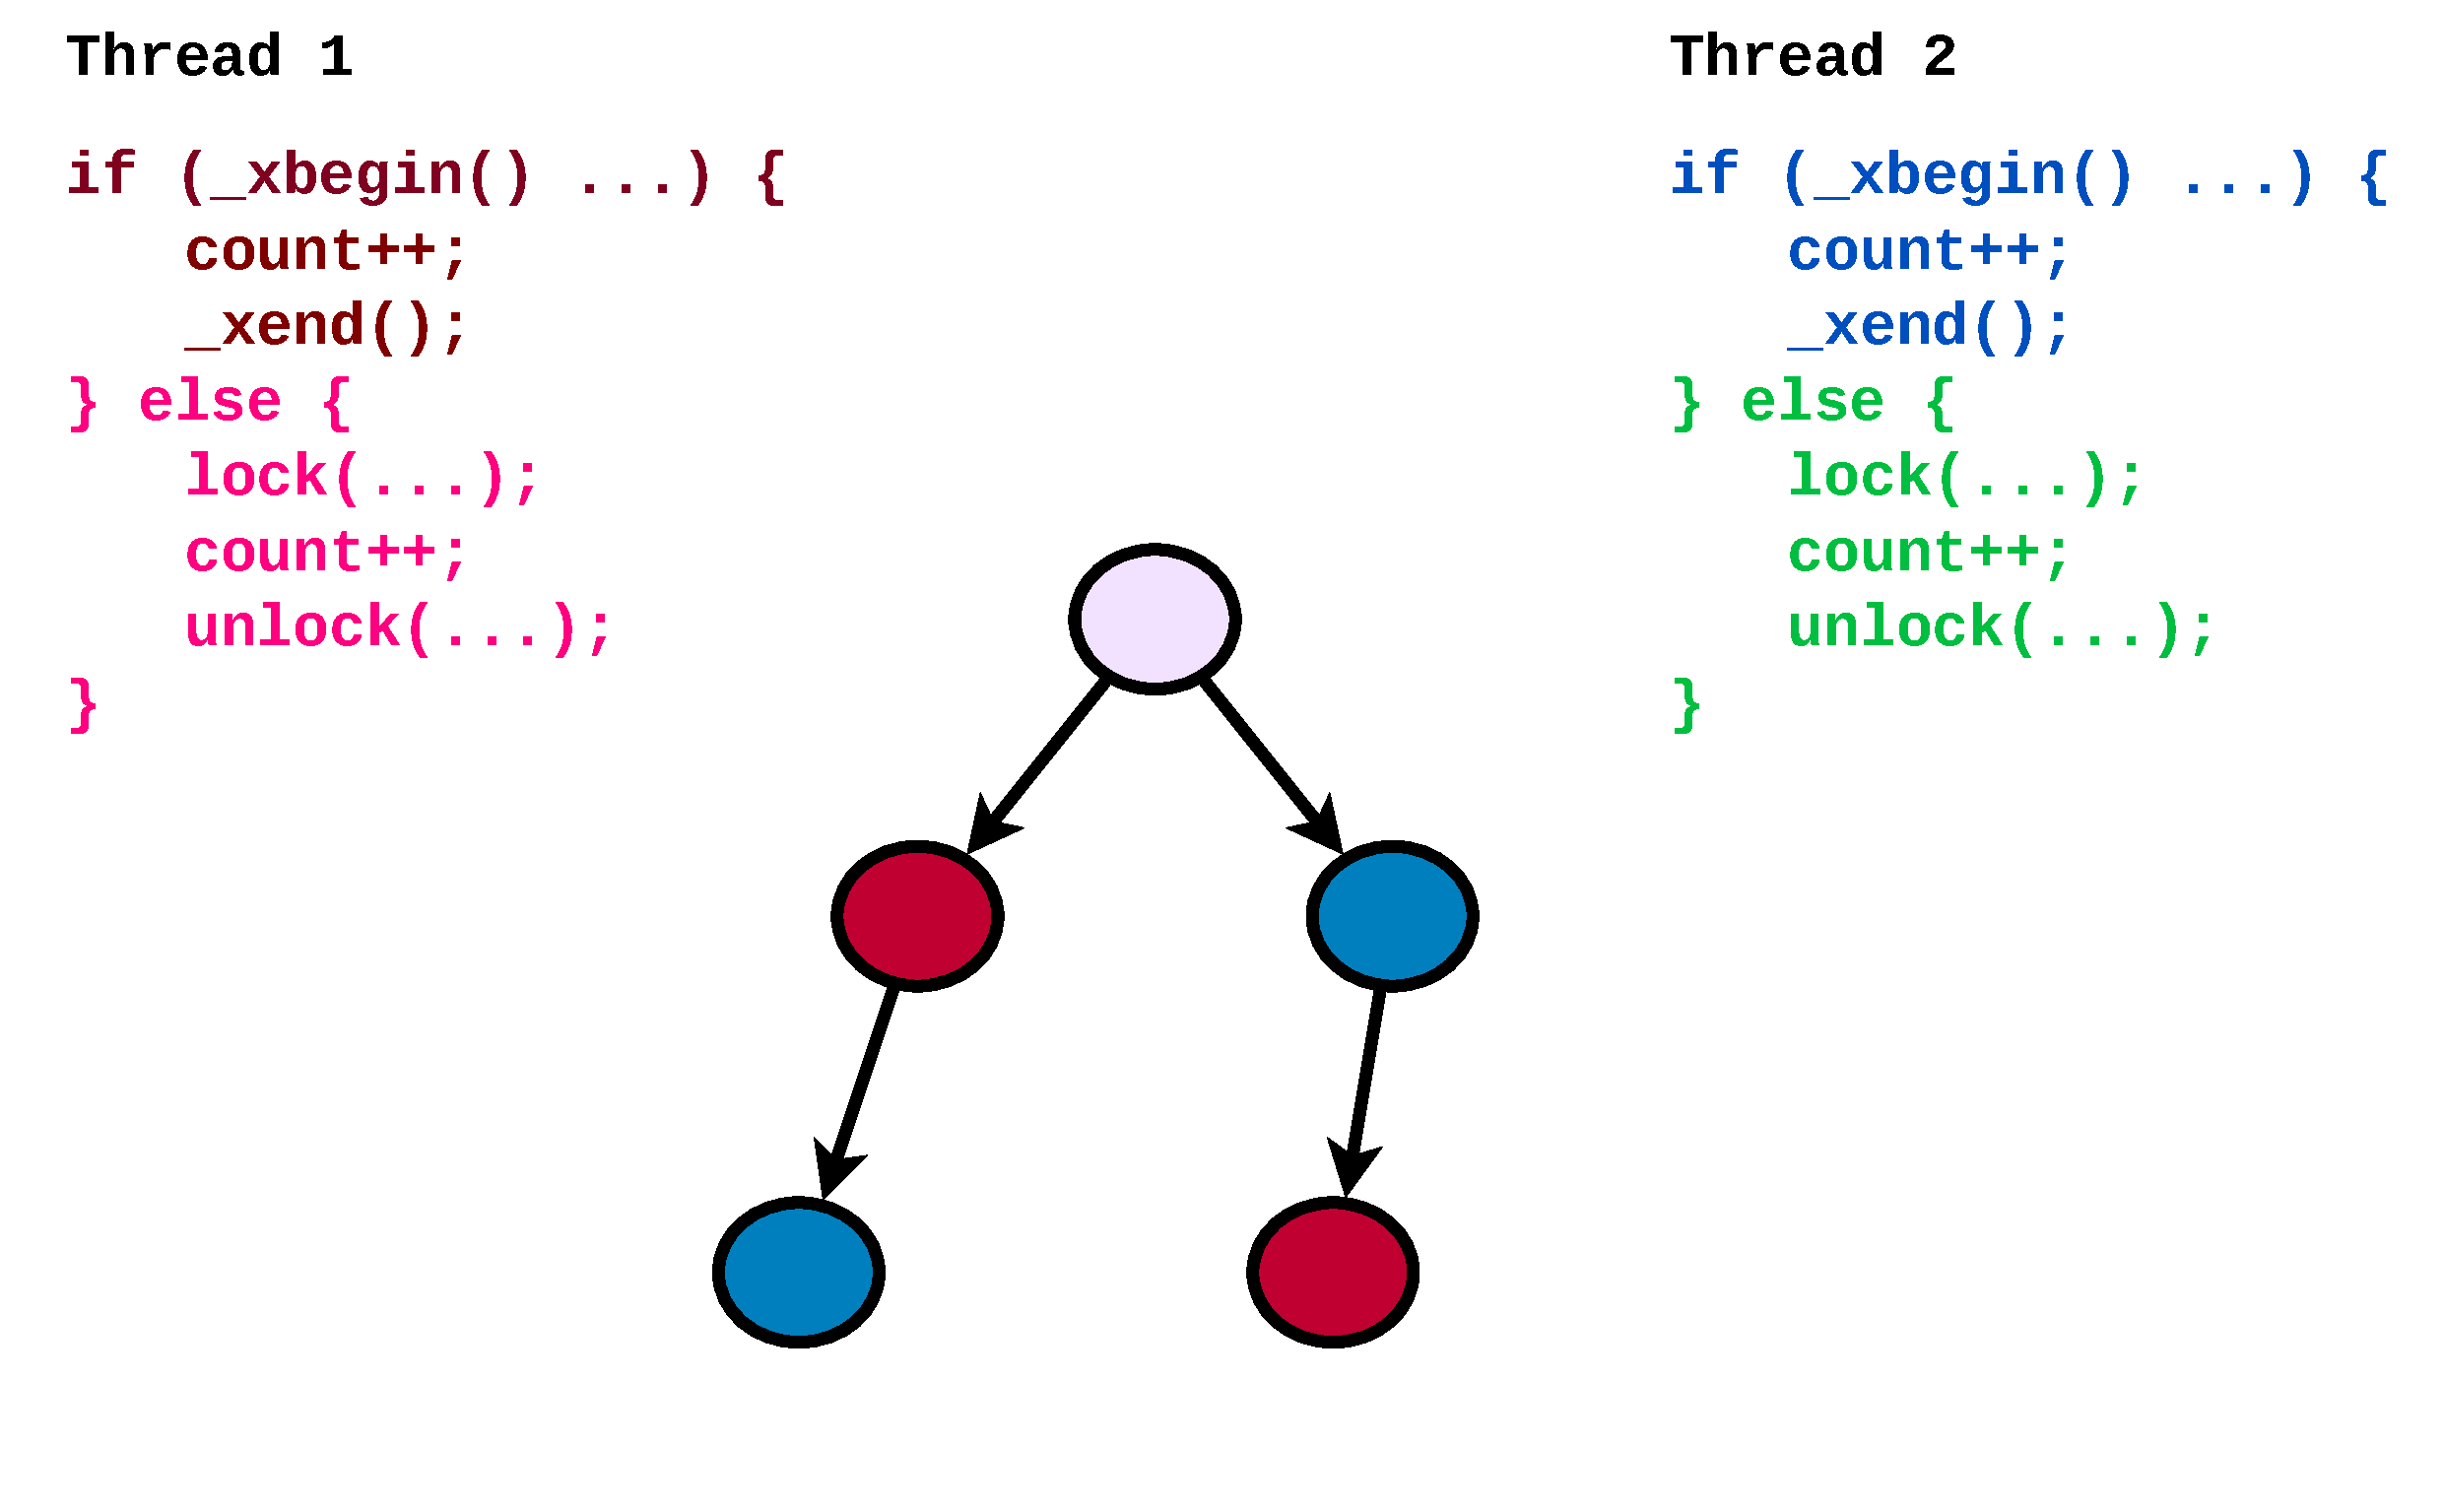
\includegraphics[width=\textwidth]{failure-injection-0.pdf}
	\end{center}
\end{frame}
\begin{frame}{Failure Injection - 2 dimensions of concurrency}
	\begin{center}
		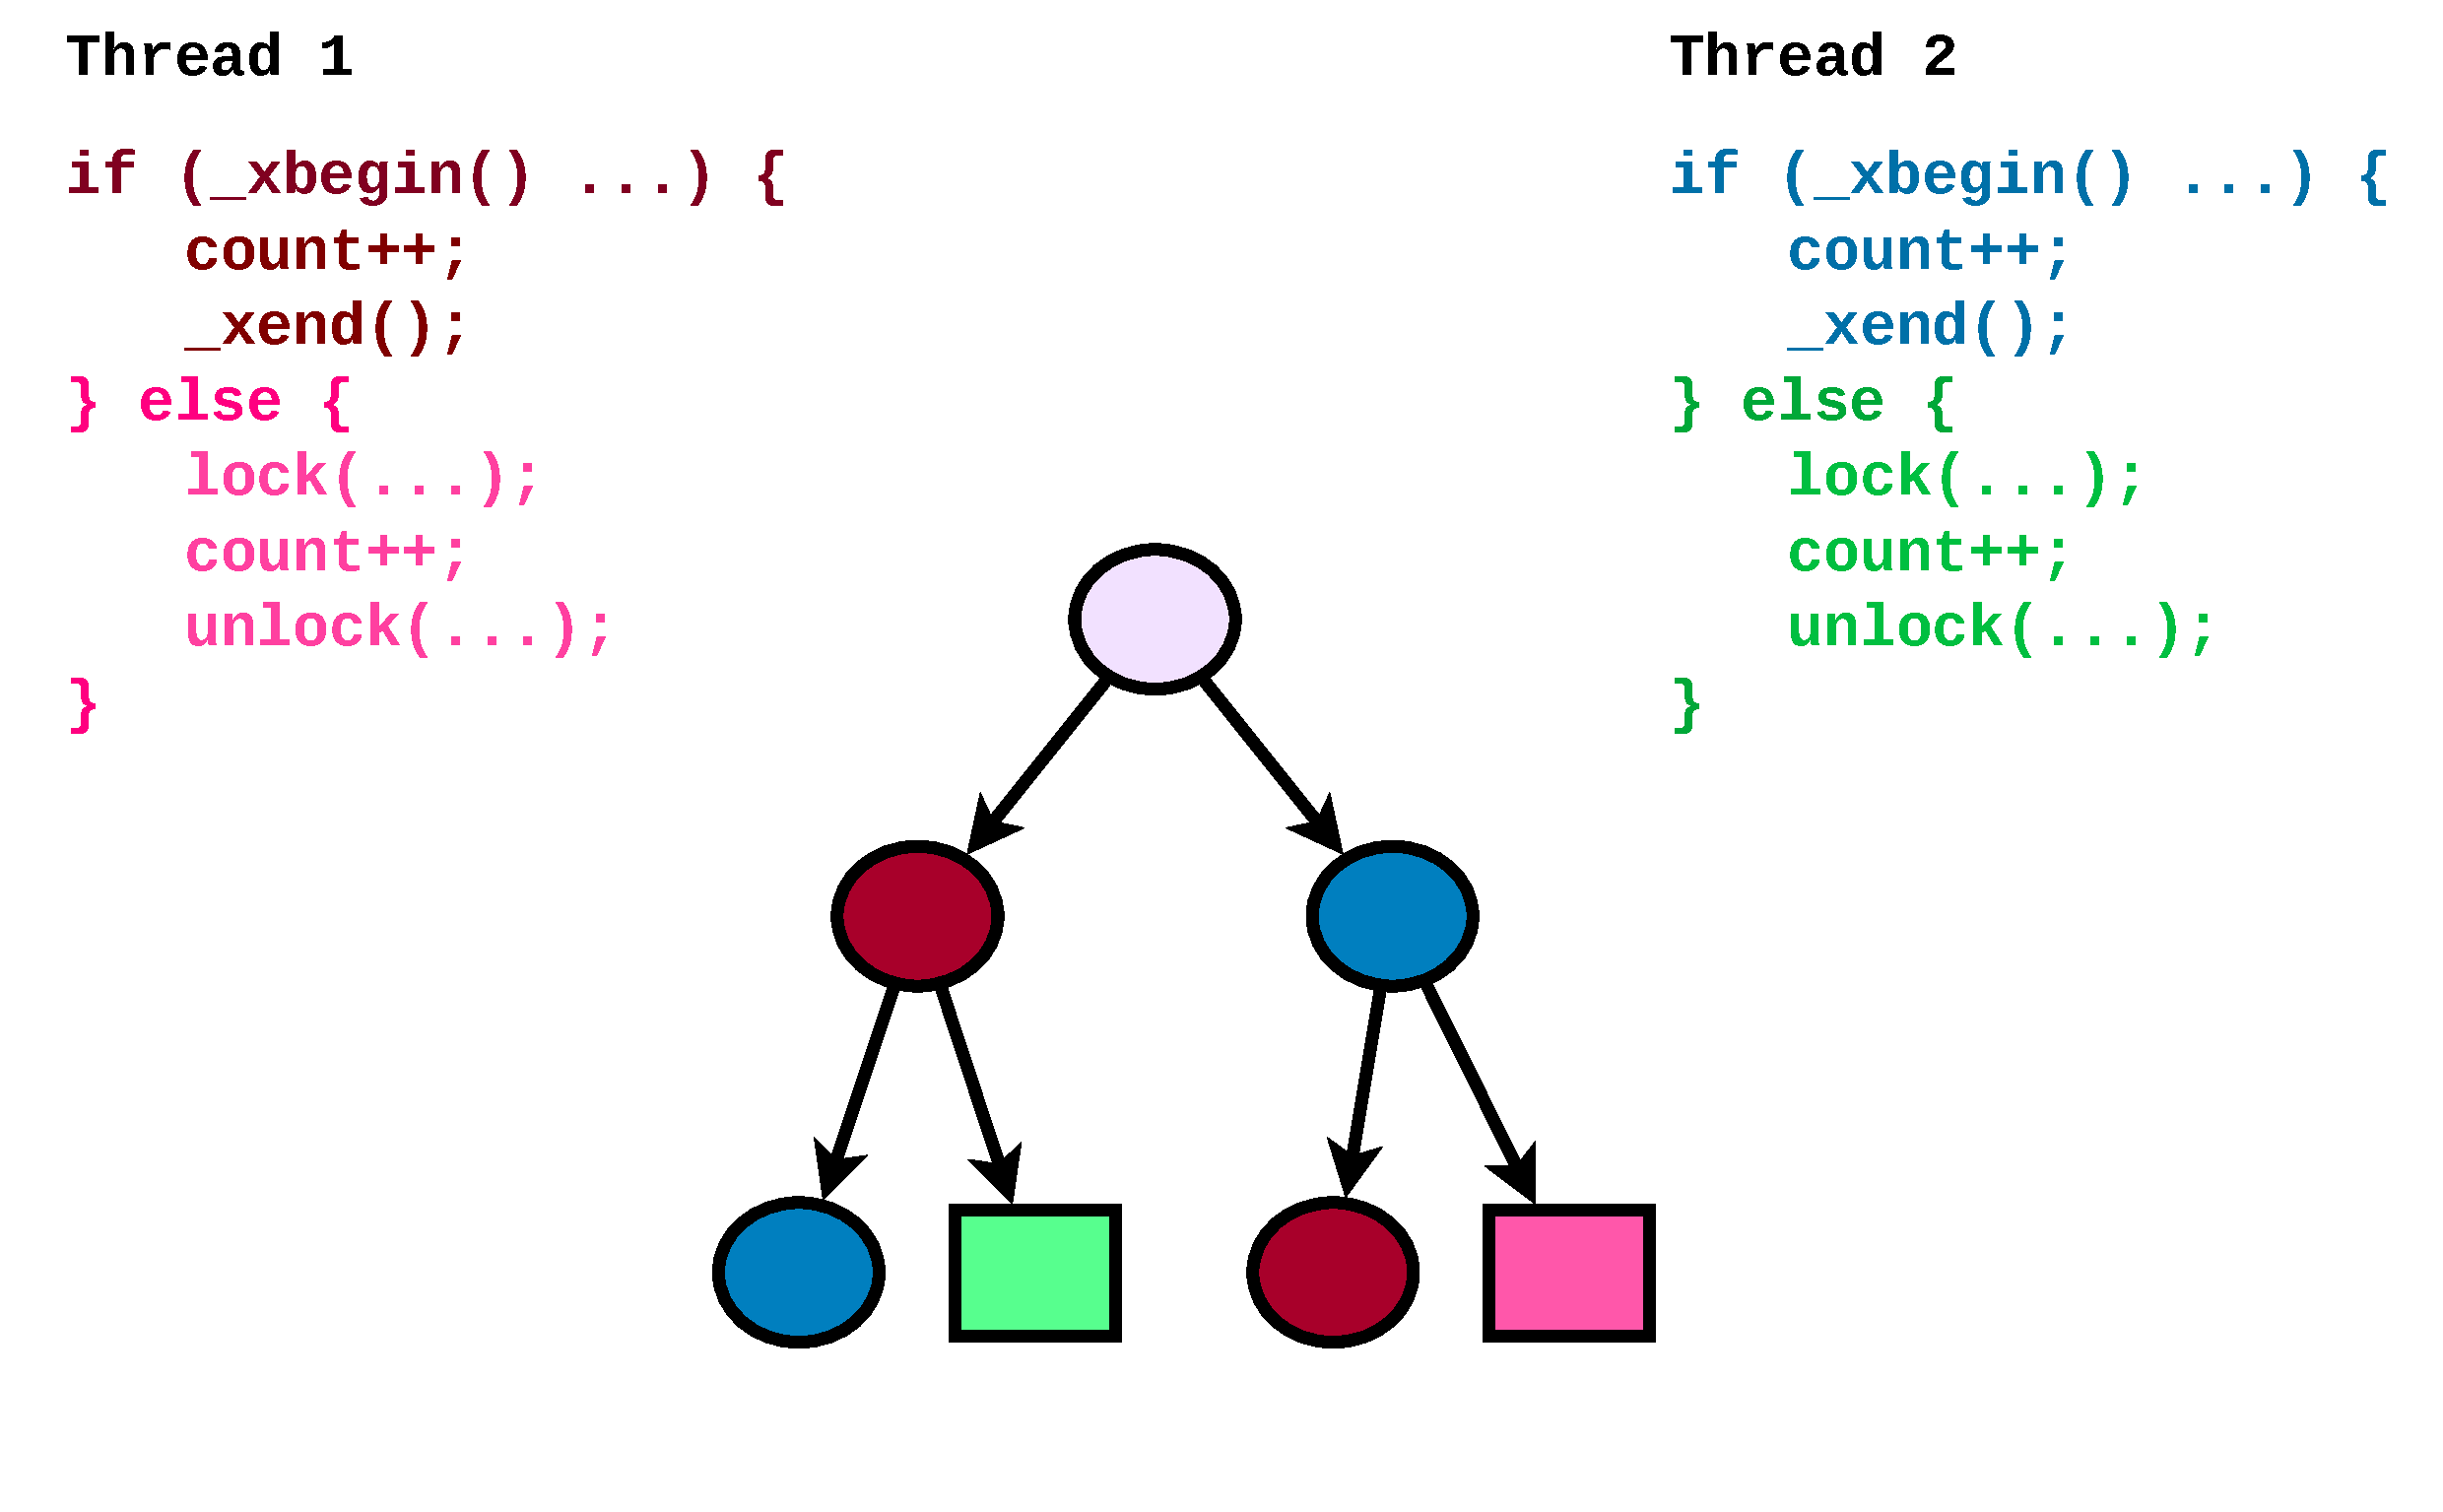
\includegraphics[width=\textwidth]{failure-injection-1.pdf}
	\end{center}
\end{frame}
\begin{frame}{Failure Injection - 2 dimensions of concurrency}
	\begin{center}
		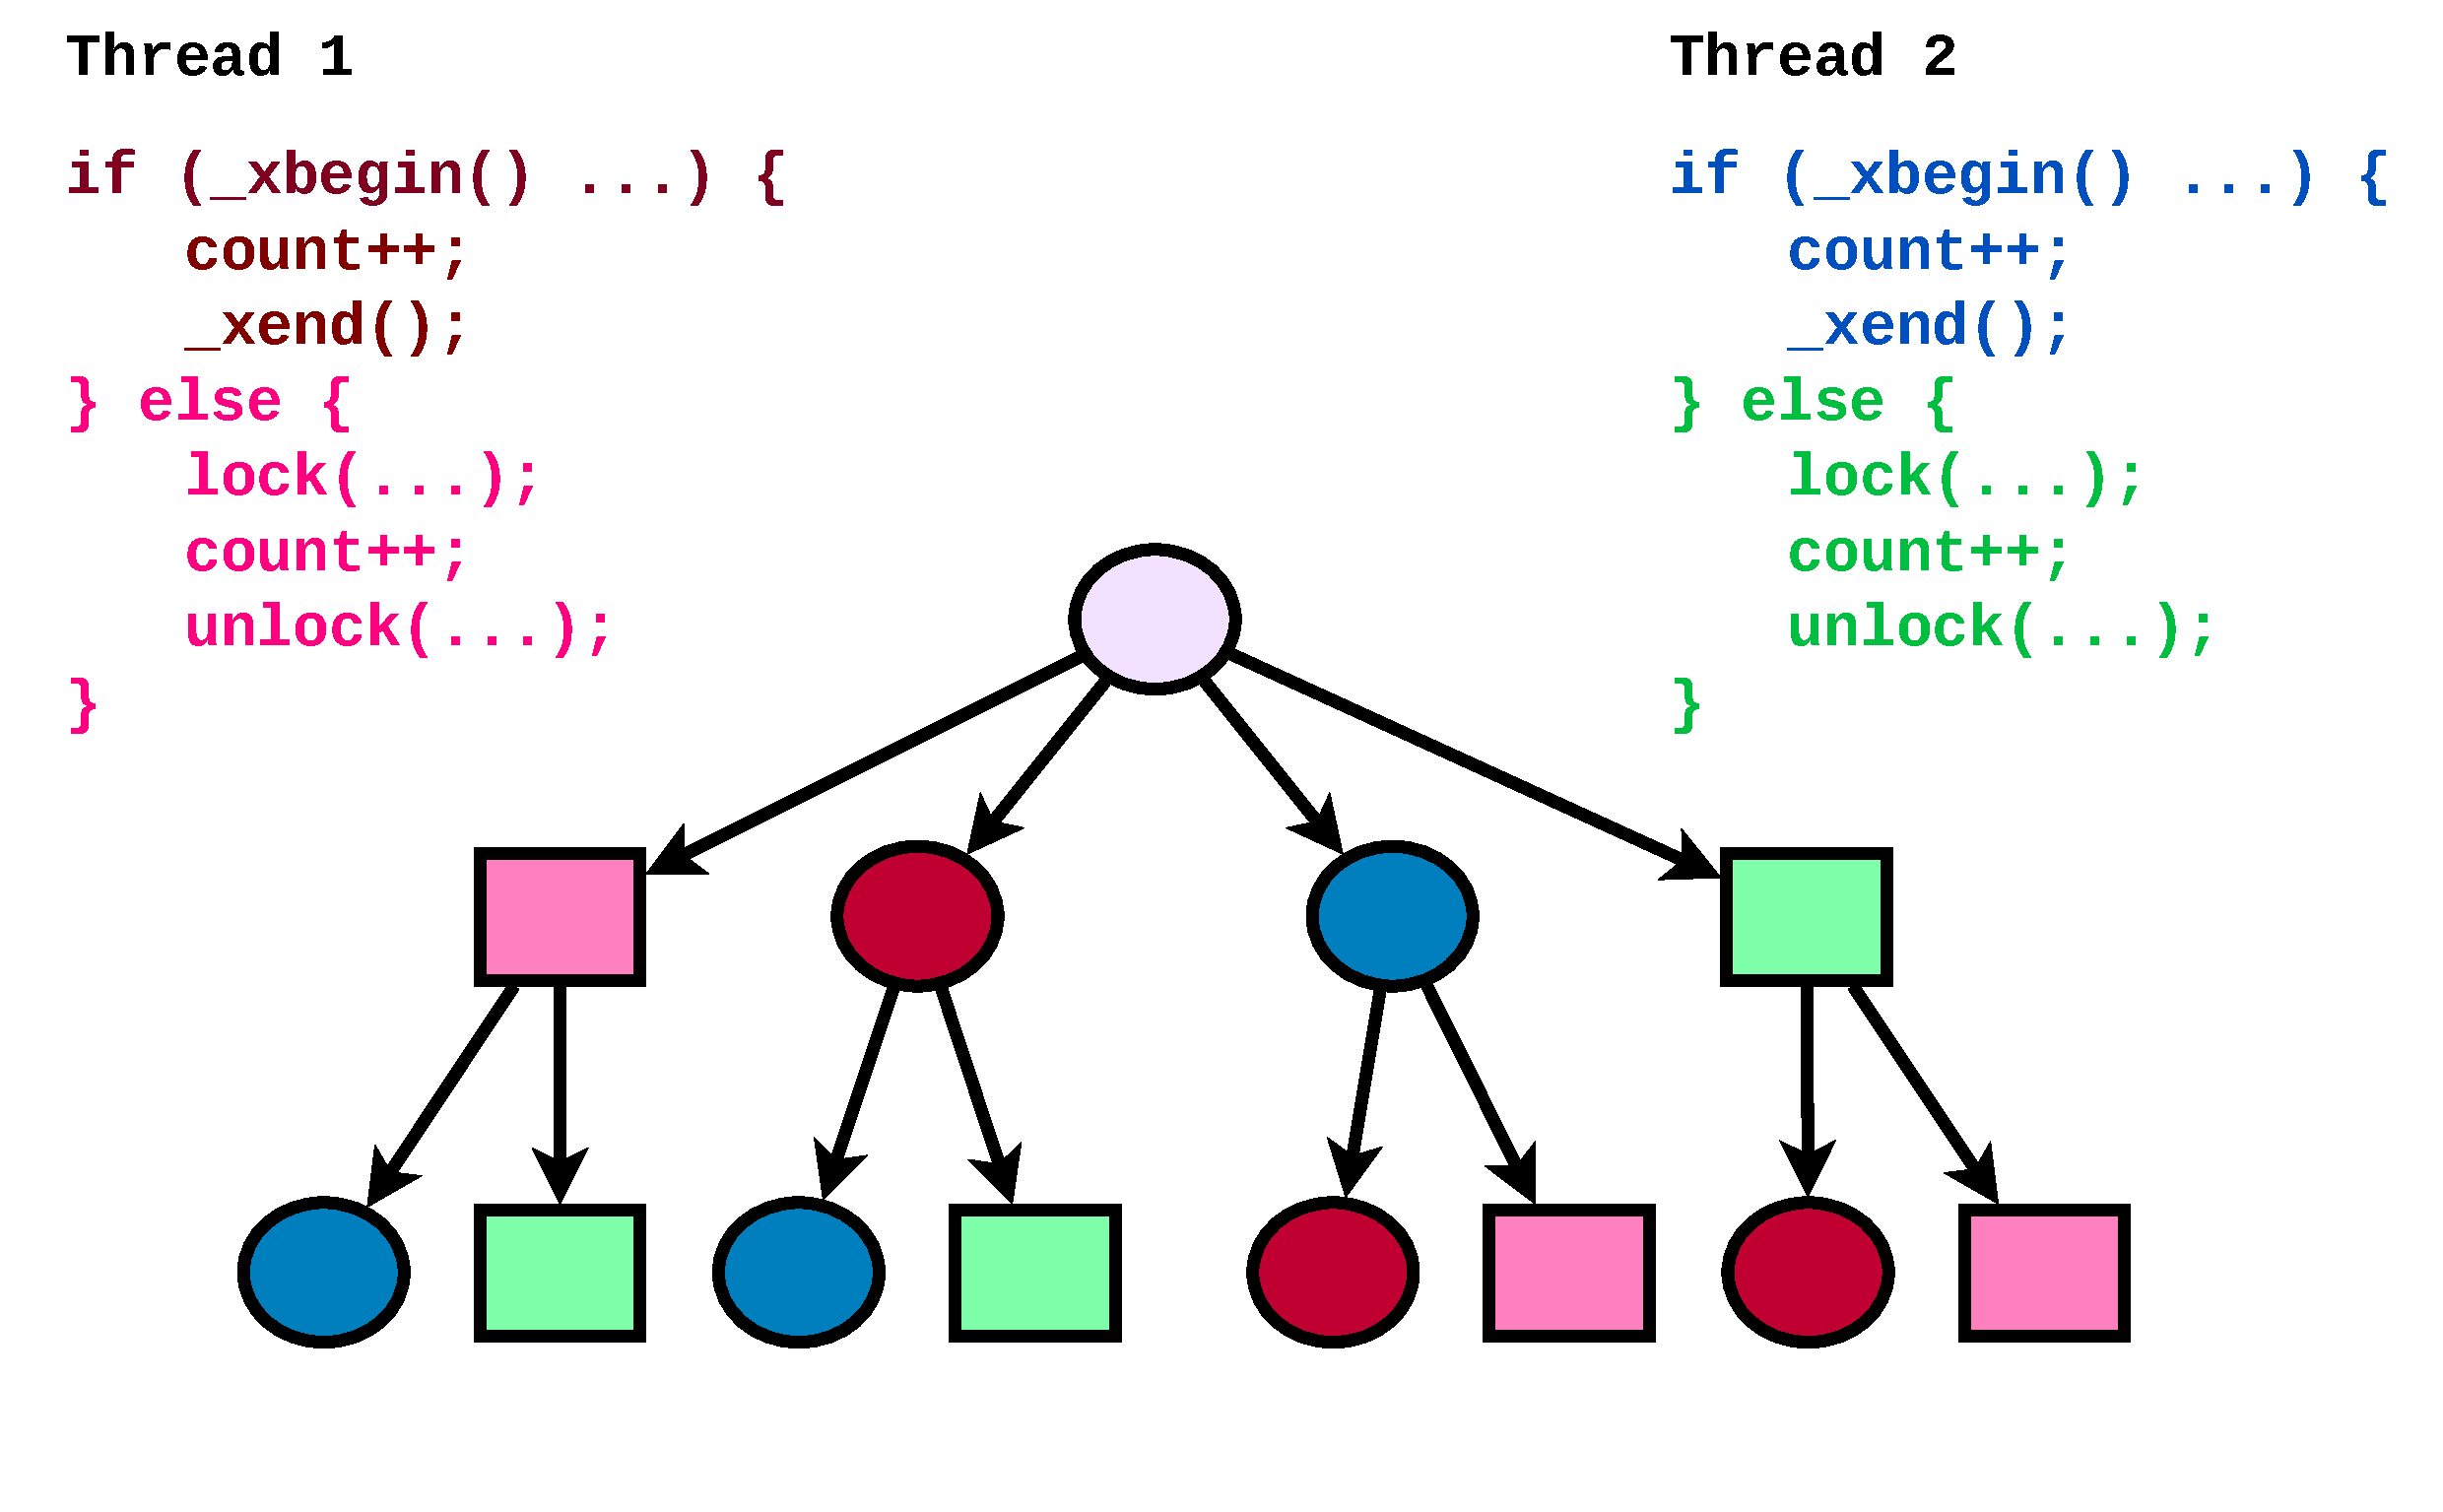
\includegraphics[width=\textwidth]{failure-injection-2.pdf}
	\end{center}
\end{frame}

\begin{frame}{Example bug}
	\begin{center}
		\begin{tabular}{l|l}
			{\bf Thread 1} & {\bf Thread 2} \\
			\hline
			{\tt \hilight{darkorange}{\_xbegin}() == ABORTED} \\
			{\tt \hilight{darkorange}{mutex\_lock}(...);} \\
			{\tt count++;} \\
			{\tt \hilight{darkblue}{mutex\_unlock}(...);} \\
				& {\tt \hilight{darkorange}{\_xbegin}() == SUCCESS} \\
				& {\tt count++;} \\
				& {\tt \hilight{darkblue}{\_xend}();} \\
			\\
			\\
		\end{tabular}
	\end{center}
\end{frame}

\begin{frame}{Example bug}
	\begin{center}
		\begin{tabular}{l|l}
			{\bf Thread 1} & {\bf Thread 2} \\
			\hline
			{\tt \hilight{darkorange}{\_xbegin}() == ABORTED} \\
			{\tt \hilight{darkorange}{mutex\_lock}(...);} \\
			{\tt int tmp = count;} \\
			{\em \hilight{pinkish}{<data-race PP>}} \\
				& {\tt \hilight{darkorange}{\_xbegin}() == SUCCESS} \\
				& {\tt count++;} \\
				& {\tt \hilight{darkblue}{\_xend}();} \\
			{\tt count = tmp + 1;} \\
			{\tt \hilight{darkblue}{mutex\_unlock}(...);} \\
		\end{tabular}
	\end{center}
\end{frame}

\begin{frame}{Example bug - Solution {\em [Dehesa-Azuara '16]}}
	\begin{center}
		\begin{tabular}{l}
			\texttt{if (\hilight{darkorange}{\_xbegin}() == SUCCESS) \{} \\ %\_XBEGIN\_STARTED) \{} \\
			%\texttt{} \\
			%\texttt{} \\
			\texttt{~~~~\hilight{pinkish}{if (mutex\_is\_locked(\&count\_lock))}} \\
			\texttt{~~~~~~~~\hilight{pinkish}{\_xabort();}} \\
			\texttt{~~~~count++;} \\
			\texttt{~~~~\hilight{darkblue}{\_xend}();} \\
			\texttt{\} else \{}\\ %if (status != \_XABORT\_EXPLICIT) \{} \\
			\texttt{~~~~\hilight{darkorange}{mutex\_lock}(\&count\_lock);} \\
			\texttt{~~~~count++;} \\
			\texttt{~~~~\hilight{darkblue}{mutex\_unlock}(\&count\_lock);} \\
			\texttt{\}} \\
		\end{tabular}
	\end{center}
\end{frame}

\begin{frame}{Example bug - Solution {\em [Dehesa-Azuara '16]}}
	\begin{center}
		\begin{tabular}{l|l}
			{\bf Thread 1} & {\bf Thread 2} \\
			\hline
			{\tt \hilight{darkorange}{\_xbegin}() == ABORTED} \\
			{\tt \hilight{darkorange}{mutex\_lock}(...);} \\
			{\tt int tmp = count;} \\
			{\em \hilight{pinkish}{<data-race PP>}} \\
				& {\tt \hilight{darkorange}{\_xbegin}() == SUCCESS} \\
				& {\tt \hilight{pinkish}{if (mutex\_is\_locked(...))}} \\
				& {\tt \hilight{pinkish}{~~~~\_xabort();}} \\
			{\tt count = tmp + 1;} \\
			{\tt \hilight{darkblue}{mutex\_unlock}(...);} \\
				& {\tt \hilight{darkorange}{mutex\_lock}(...);} \\
				& {\tt count++;} \\
				& {\tt \hilight{darkblue}{mutex\_unlock}(...);} \\
		\end{tabular}
	\end{center}
\end{frame}


\begin{frame}{Evaluation}
	Questions
	\begin{itemize}
		\item Does Landslide find previously-unknown bugs in HTM programs?
		\item Does Landslide verify HTM code in reasonable time?
	\end{itemize}
	\linegap

	Test suite
	\begin{itemize}
		\item Hand-written unit tests
		\item Transactional data structures {\em [Dehesa-Azuara '16]}
		\item Spinlock from TSX LevelDB implementation {\em [vamsikc '14]}
	\end{itemize}
\end{frame}

\begin{frame}{Evaluation - Bug-finding}
	Example - {\tt count++} data race
	\begin{itemize}
		\item Landslide finds assertion failure in 7 seconds % 2,1 with -M, 5 interleavings, wall clock time
	\end{itemize}
	\linegap

	AVL tree - atomicity violation
	\begin{itemize}
		\item Forgot the {\tt mutex\_is\_locked()} check $\rightarrow$ data corruption
		\item Landslide finds segfault in 15 seconds % 3,1 with quicksand; 14 interleavings, wall clock time
		%\item Same author who proposed the fix... % this bullet exists in summary slide
	\end{itemize}
	\linegap

	Spinlock - performance degradation
	\begin{itemize}
		\item {\tt mutex\_is\_locked()} used {\tt cmpxchg} (= atomic read + write)
		\item Unconditional write during {\tt xbegin} path $\rightarrow$ always aborts!
		\item Landslide finds assertion failure in 3 seconds % 2,2 with -M, 2 interleavings, wall clock time
	\end{itemize}
\end{frame}

\begin{frame}{Evaluation - Verification}
	$K,N$ = $K$ threads, each $N$ iterations of test logic; 10 hour timeout
	\linegap

	Microbenchmarks
	\begin{itemize}
			% numbers taken from retry sets column
		\item {\tt mutex\_is\_locked()} pattern: $K,N$ = 2,4 (79min); 4,1 (6min)
		%\item Using {\tt xadd} instead: $K,N$ = 2,4 (19min); 3,2 (39min), 4,1 (1min)
		\item (more tests in thesis)
		\item Is that ``enough''? Generalize with manual inspection?
	\end{itemize}
	\pause
	\linegap

	HTM data structures
	\begin{itemize}
			% numbers taken from retry sets column
		\item Hashmap insert: $K,N$ = 2,1 (27sec) % map_basicer. not dealing with resizing here
		\item AVL tree insert: $K,N$ = 2,1 (5min)
			\pause
		\begin{itemize}
			\item but... requires $K \times N \ge 3$ to expose the segfault...
			\begin{itemize}
				\item Estimated time for $K,N$ = 3,1... 736 years...
					% 2,2 -> 51000 years lmao
			\end{itemize}
		\end{itemize}
	\end{itemize}

\end{frame}

\begin{frame}{Evaluation - Verification}
	Abstraction reduction {\em [Simsa '13]}
	\begin{itemize}
		\item Verify locking primitives \& client code separately against common API
			% say: again relying on human to write the right test case
		\item {\em Add} verification costs instead of {\em multiplying}
	\end{itemize}
	\linegap

	HTM locks
	\begin{itemize}
			% numbers are now using STM semantics instead
			% bc of retry loop around the xbegin
			% can't really mention this in the talk
		\item Spinlock: $K,N$ = 2,2 (2min), 3,1 (28sec)
			\begin{itemize}
				\item Depends on ad-hoc yield-loop heuristics; slow
			\end{itemize}
		\item Spin replaced w/P2 mutex: $K,N$ = 2,4 (7hrs), 4,1 (11min)
	\end{itemize}
	\pause
	\linegap

	HTM data structures w/verified locks
	\begin{itemize}
		\item Hashmap insert: $K,N$ = 2,3 (4hrs), 3,1 (11min)
		\item AVL tree insert: $K,N$ = 2,4 (4min), 3,2 (23min), 4,1 (3min)
	\end{itemize}
\end{frame}

\begin{frame}{Summary}
	HTM adds new ``dimension'' of concurrency
	\begin{itemize}
		\item Equivalence theorem lets Landslide emulate execution semantics
		\item Allows exponential reduction of non-observable behaviours
	\end{itemize}
	\linegap

	Even simple programs tricky to get right
	\begin{itemize}
		\item Author of {\tt mutex\_is\_locked()} pattern got it wrong once...
		\item Landslide can check even unpredictable performance characteristics
	\end{itemize}
	\linegap

	Abstraction reduction eases both implementation \& verification burden
\end{frame}

%%%%%%%%%%%%%%%%%%%%%%%%%%%%%%%%%%%%%%%%%%%%%%%%%%%%%%%%%%%%%%%%%%%%%%%%%%%%%%%%
%%%%%%%%%%%%%%%%%%%%%%%%%%%%%%%%%%%%%%%%%%%%%%%%%%%%%%%%%%%%%%%%%%%%%%%%%%%%%%%%
%%%%%%%%%%%%%%%%%%%%%%%%%%%%%%%%%%%%%%%%%%%%%%%%%%%%%%%%%%%%%%%%%%%%%%%%%%%%%%%%

\section{Part 4}
\subsection{End}

\breakslide{\Large \bf Conclusion}

\begin{frame}{Conclusion}
	% data race pps (as well as txn equivalence)
	Combining %both
	theoretically-founded automatic reduction techniques
	% iterative deepening
	% (say smth like: "landslide also has a wealth of other user-tunable heuristics
	% for expert users, which you can read about in the document; for this talk i will focus just on the CPU budget thing")
	% XXX: need to prepare for the question -- "what evidence do you have that users actually want this cpu budget stuff",
	% ",or, that it helps vs just running something unlimited vs a normal icb test"
	% (well, for the 2nd half of the Q, i can talk about how ID outperforms ICB on verficiations)
	and user-informed heuristic ones,
	\linegap

	stateless model checking
	\hilight{sect-quicksand}{can sufficiently mitigate exponential explosion}\xspace
	\hilight{sect-410}{to be practical for inexperienced users}\xspace
	\hilight{sect-htm}{and real-world programs alike.}\xspace
\end{frame}
\begin{frame}{Conclusion}
	% data race pps (as well as txn equivalence)
	Combining %both
	{\bf theoretically-founded automatic reduction techniques}
	\vspace{4.82em}

	and {\bf user-informed heuristic ones},
	\vspace{4.82em}
	\linegap

	stateless model checking
	\hilight{sect-quicksand}{can sufficiently mitigate exponential explosion}\xspace
	\hilight{sect-410}{to be practical for inexperienced users}\xspace
	\hilight{sect-htm}{and real-world programs alike.}\xspace
\end{frame}
\begin{frame}{Conclusion}
	%\hilight{gray}{Combining %both
	%{\bf theoretically-founded automatic reduction techniques}}
	Combining %both
	{\bf theoretically-founded automatic reduction techniques}
	\begin{itemize}
		\item \hilight{sect-quicksand}{Verification with data-race preemption points}
		\item \hilight{sect-410}{Student yield-loop blocking} % student (adj). from "studence"
		\item \hilight{sect-htm}{Equivalent emulation of HTM semantics}
	\end{itemize}
	% TODO: incremental reveal
	%\hilight{gray}{and {\bf user-informed heuristic ones},}
	and {\bf user-informed heuristic ones},
	\begin{itemize}
		\item \hilight{sect-quicksand}{Quicksand's CPU budget argument}
		\item \hilight{sect-410}{Exposing data-race reports to students}
		%\item Encouraging students to exercise their intuition % ??
		\item \hilight{sect-htm}{Abstraction reduction for HTM primitives}
	\end{itemize}
	\linegap

	\hilight{gray}{stateless model checking}\xspace
	\hilight{sect-pastel-quicksand}{can sufficiently mitigate exponential explosion}\xspace
	\hilight{sect-pastel-410}{to be practical for inexperienced users}\xspace
	\hilight{sect-pastel-htm}{and real-world programs alike.}\xspace
\end{frame}
\begin{frame}{Closing remarks}
	``Verifying C programs is doomed, why can't PL design handle this?''
	\begin{itemize}
		\item seL4 {\em [Klein '09]}: secure kernel verified end-to-end in Haskell
		\item Rust {\em [Matsakis '14]}: concurrency-aware type system, no data races
	\end{itemize}
	\pause
	\linegap

	But... we still have to try.
	\begin{itemize}
		\item Computers can't handle $O(N^K)$
			\begin{itemize}
				\item ``ok, $N^K$, that's, wow, 700 years...''
			\end{itemize}
		\item Humans can help?
			\begin{itemize}
				\item ``can we get same results with smaller $N$, $K$?''
			\end{itemize}
	\end{itemize}
	\pause
	\linegap

	One day live in peace with our silicon children?
\end{frame}

\breakslide{
\begin{center}
	% TODO: replace with HIL for honban
	\Large Q\&A
	%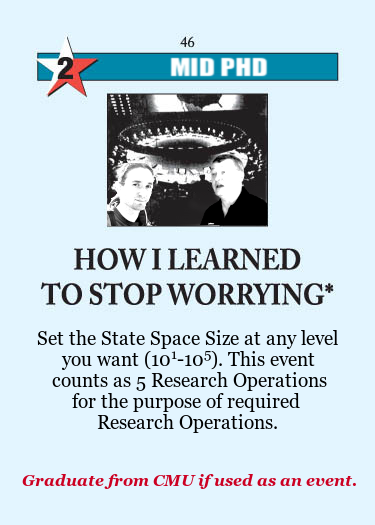
\includegraphics[width=0.4\textwidth]{../how-i-learned.png}
\end{center}
%\linegap
%
%\begin{center}
%	\includegraphics[width=0.65\textwidth]{3word-questions.png}
%\end{center}
}

%%%%%%%%%%%%%%%%%%%%%%%%%%%%%%%%%%%%%%%%%%%%%%%%%%%%%%%%%%%%%%%%%%%%%%%%%%%%%%%%
%%%%%%%%%%%%%%%%%%%%%%%%%%%%%%%%%%%%%%%%%%%%%%%%%%%%%%%%%%%%%%%%%%%%%%%%%%%%%%%%
%%%%%%%%%%%%%%%%%%%%%%%%%%%%%%%%%%%%%%%%%%%%%%%%%%%%%%%%%%%%%%%%%%%%%%%%%%%%%%%%

\section{Warp Zone}

\subsection{Quicksand}
\breakslide{\Large \bf \hilight{sect-quicksand}{Bonus Slides - Quicksand}}

\begin{frame}{Data-Race Definitions}
	\textbf{Data race:} 2 threads access the same memory, and...
	\begin{itemize}
		\item At least one access is a write
		\item Threads do not hold the same lock
		\item No {\em Happens-Before} relation between threads
	\end{itemize}
	\pause
	\linegap

	Variants of Happens-Before (HB)
	\begin{itemize}
		\item {\bf Pure HB:} Any synchronization events {\em [Lamport '78]}
			% Say: "Or another way of putting it I heard from one of yesterday's talks that I'm stealing, one event is guaranteed to be visible to the other"
			% Or don't, idgaf
		\item {\bf Limited HB:} Blocking synchronization (e.g. \texttt{cond\_wait()}) enforces one ordering {\em [O'Callahan '03]}
	\end{itemize}
\end{frame}

\begin{frame}{Happens-Before Example}
	\begin{center}
		\begin{tabular}{ll}
			{\bf Thread 1}  & {\bf Thread 2} \\
			\texttt{\hilight{pinkish}{x++;}}    & \\
			\texttt{mutex\_lock(m);}	& \\
			\texttt{\hilight{lavender}{// unrelated}}	   & \\
			\texttt{mutex\_unlock(m);}      & \\
				& \texttt{mutex\_lock(m);} \\
				& \texttt{\hilight{lavender}{// unrelated}} \\
				& \texttt{mutex\_unlock(m);} \\
				& \texttt{\hilight{pinkish}{x++;}} \\
		\end{tabular}
		\linegap

		No race under Pure HB; {\em true potential race} under Limited HB.
	\end{center}
\end{frame}
\begin{frame}{Happens-Before Example}
	\begin{center}
		\begin{tabular}{ll}
			{\bf Thread 1}  & {\bf Thread 2} \\
			\texttt{\hilight{pinkish}{x++;}}    & \\
			\texttt{mutex\_lock(m);}	& \\
			\texttt{\hilight{lavender}{y = true;}}      & \\
			\texttt{mutex\_unlock(m);}      & \\
				& \texttt{mutex\_lock(m);} \\
				& \texttt{\hilight{lavender}{bool tmp = y;}} \\
				& \texttt{mutex\_unlock(m);} \\
				& \texttt{\hilight{lavender}{if (tmp)}~\hilight{pinkish}{x++;}} \\
		\end{tabular}
		\linegap

		No race under Pure HB; {\em false positive} under Limited HB.
	\end{center}
\end{frame}

\begin{frame}{Quicksand (Iterative Deepening) Reductions}
	If one job is a subset of another, testing either might let us skip the other.
	\begin{center}
		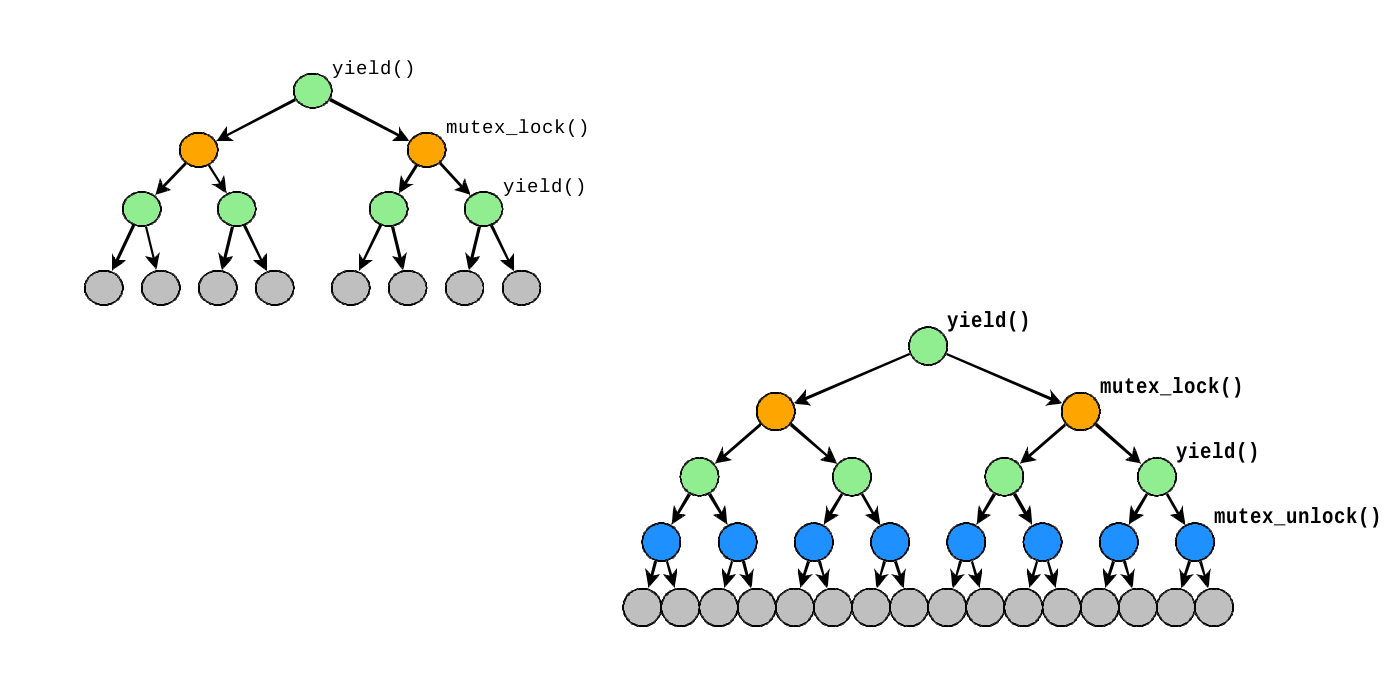
\includegraphics[width=\textwidth]{../../oopsla/reduction-nothing.png}
	\end{center}
\end{frame}
\begin{frame}{Quicksand (Iterative Deepening) Reductions}
	If one job is a subset of another, testing either might let us skip the other.
	\begin{center}
		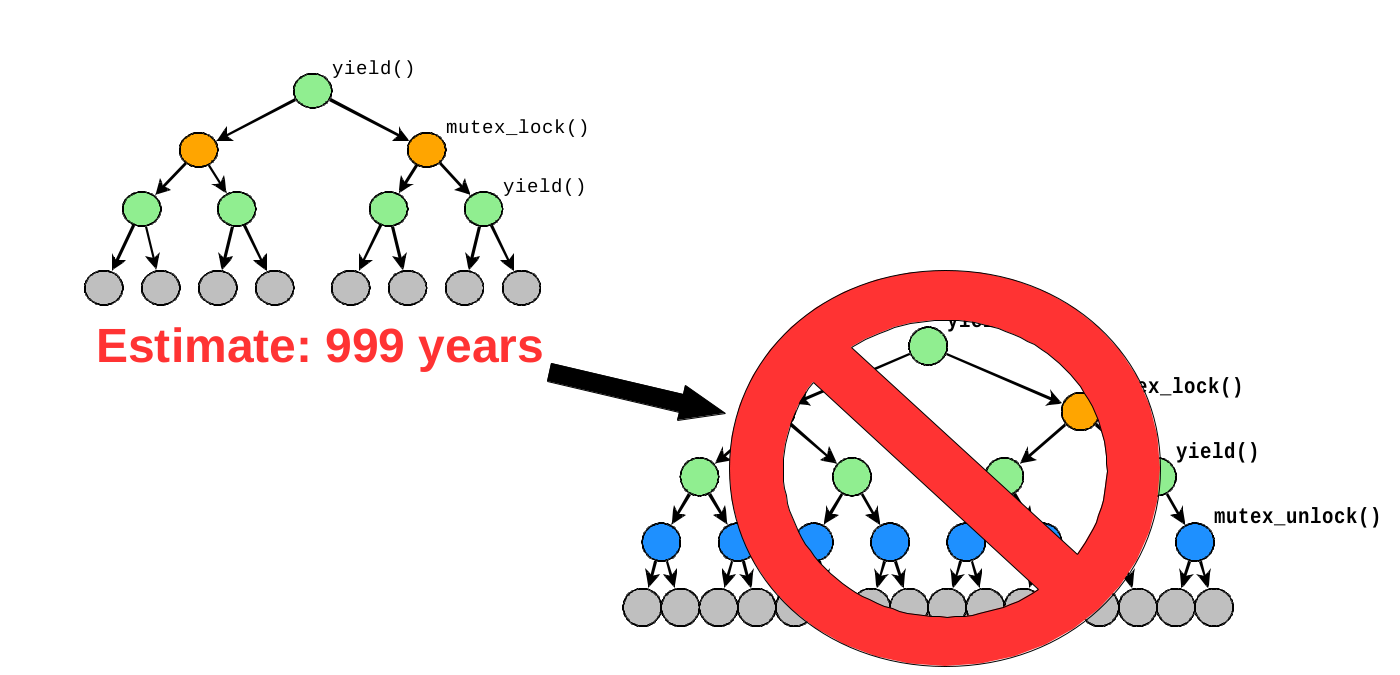
\includegraphics[width=\textwidth]{../../oopsla/reduction-deferred.png}
	\end{center}
\end{frame}
\begin{frame}{Quicksand (Iterative Deepening) Reductions}
	If one job is a subset of another, testing either might let us skip the other.
	\begin{center}
		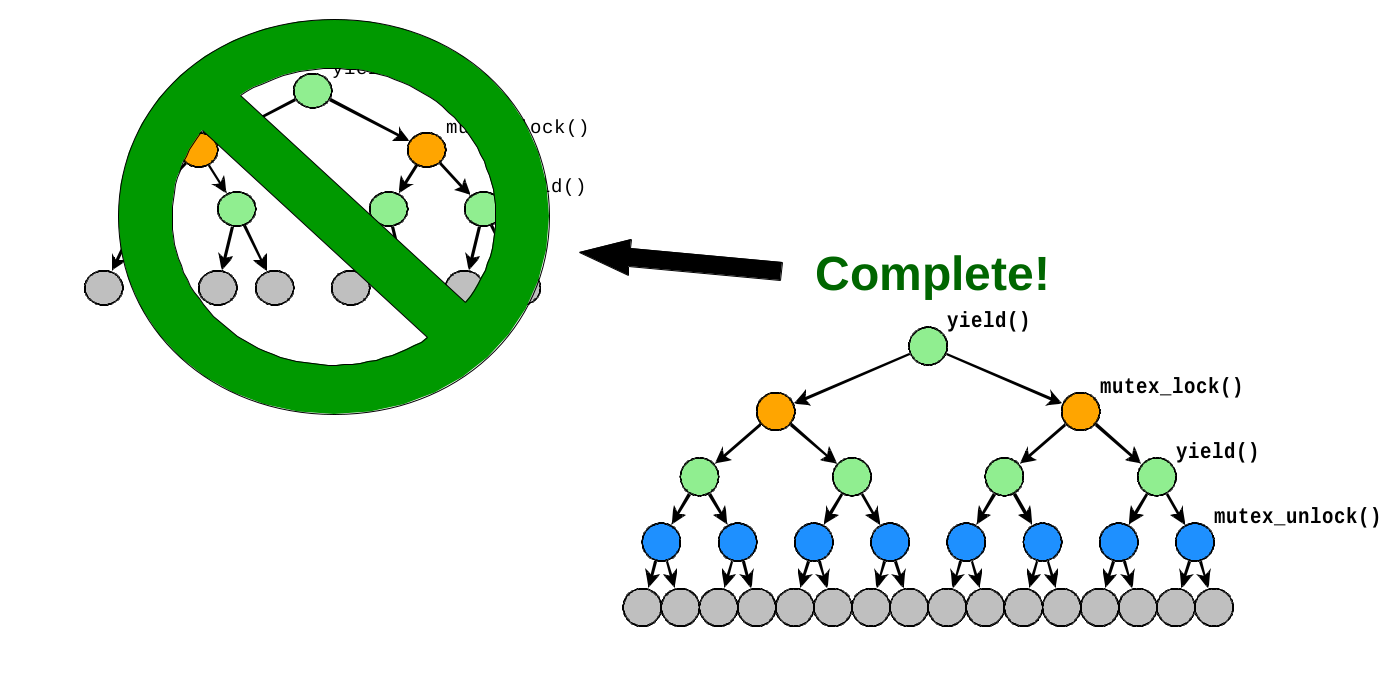
\includegraphics[width=\textwidth]{../../oopsla/reduction-complete.png}
	\end{center}
\end{frame}

\begin{frame}{Quicksand results - Bugs found by CPU time}
	\begin{center}
		\includegraphics[width=0.8\textwidth]{../quicksand-bugs-hb-talkver.pdf}
	\end{center}
\end{frame}
\begin{frame}{Quicksand results - Bugs found by wall-clock time}
	\begin{center}
		\includegraphics[width=0.8\textwidth]{../quicksand-bugs-hb-wallclock-talkver.pdf}
	\end{center}
\end{frame}
\begin{frame}{Quicksand results - Tests fully verified (CPU time)}
	\begin{center}
		\includegraphics[width=0.8\textwidth]{../quicksand-verifs-hb-talkver.pdf}
	\end{center}
\end{frame}
\begin{frame}{Quicksand results - MC + DR vs single-pass DR}
	\begin{center}
		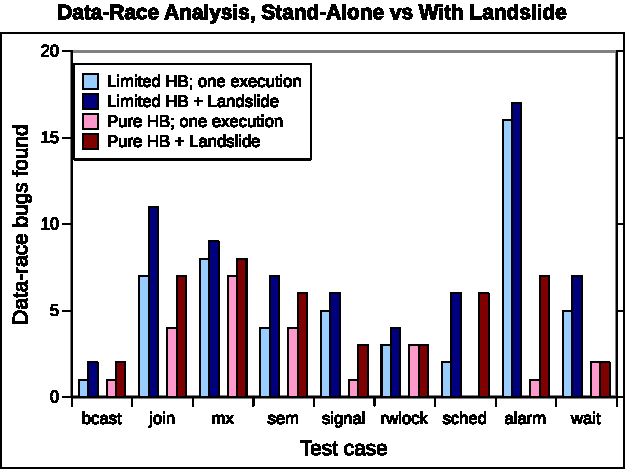
\includegraphics[width=0.8\textwidth]{../../oopsla/dr-false-negatives-poster.pdf}
	\end{center}
\end{frame}
\begin{frame}{Quicksand results - Representative of real-world programs?}
	Bugs by required number of preemptions to expose:
	\begin{center}
		\footnotesize
	\begin{tabular}{r|c|c}
		{\bf Bound} & {\bf ICB (sync PPs only)} & {\bf ICB (preempt everywhere)} \\
		\hline
		0       & 2     & 1     \\
		1       & 82    & 86    \\
		2       & 16    & 32    \\
		3       & 2     & 3     \\
		4+      & 0     & 0     \\
		\hline
		Total   & 102   & 122   \\
	\end{tabular}
	\end{center}
	\linegap

	Bugs by type (Pure HB Quicksand):
	\begin{itemize}
		\item 56 deadlocks
		\item 49 heap errors (47 use-after-free)
		\item 35 assertion failures
		\item 31 page/segmentation fault crashes
		\item 1 infinite loop
		\item 1 recursive mutex lock
	\end{itemize}
\end{frame}

%%%%%%%%%%%%%%%%%%%%%%%%%%%%%%%%%%%%%%%%%%%%%%%%%%%%%%%%%%%%%%%%%%%%%%%%%%%%%%%%
\subsection{Education}
\breakslide{\Large \bf \hilight{sect-410}{Bonus Slides - Education}}

\begin{frame}{15-410...}
	% TODO:
	% study of tej/etc specific bugs
	% list tests cases provided to studence & PSU-specific ones too
\end{frame}

%%%%%%%%%%%%%%%%%%%%%%%%%%%%%%%%%%%%%%%%%%%%%%%%%%%%%%%%%%%%%%%%%%%%%%%%%%%%%%%%
\subsection{HTM}
\breakslide{\Large \bf \hilight{sect-htm}{Bonus Slides - HTM}}

\begin{frame}{HTM: Even more dimensions of nondeterminism}
	% The gotcha: When xbegin can fail, it can emit diff error codes, which depend on what happened within.
	\begin{center}
		\begin{tabular}{l}
			\texttt{if ((status = \hilight{darkorange}{\_xbegin}()) == \_XBEGIN\_STARTED) \{} \\
			\texttt{~~~~if (count >= 100)}\\
			\texttt{~~~~~~~~\hilight{pinkish}{\_xabort}();} \\
			\texttt{~~~~count++;} \\
			\texttt{~~~~\hilight{darkblue}{\_xend}();} \\
			\texttt{\} else if (status != \_XABORT\_EXPLICIT) \{} \\
			\texttt{~~~~\hilight{darkorange}{mutex\_lock}(\&count\_lock);} \\
			\texttt{~~~~count++;} \\
			\texttt{~~~~\hilight{darkblue}{mutex\_unlock}(\&count\_lock);} \\
			\texttt{\}} \\
		\end{tabular}
	\end{center}
	\linegap

	\xbegin can fail with multiple possible error codes
	\begin{itemize}
		\item MC will identify on-the-fly when (e.g.) {\tt \_XABORT\_EXPLICIT} is possible
		\item Treat such transactions as having multiple failure injection possibilities
		\item Future work: dataflow analysis to know when failure reason never used
	\end{itemize}
\end{frame}

\begin{frame}{HTM: Possible \xabort error codes}
	From GCC 4.8.2 manual \S 6.56.8, ``X86 transaction memory intrinsics'':
	\begin{itemize}
		\item {\tt \_XABORT\_EXPLICIT} - Transaction explicitely [sic] aborted with \xabort.
			%The parameter passed to \xabort is available with {\tt \_XABORT\_CODE(status)}
		\item {\tt \_XABORT\_RETRY} - Transaction retry is possible.
		\item {\tt \_XABORT\_CONFLICT} - Transaction abort due to a memory conflict with another thread
		\item {\tt \_XABORT\_CAPACITY} - Transaction abort due to the transaction using too much memory
		\item {\tt \_XABORT\_DEBUG} - Transaction abort due to a debug trap
		\item {\tt \_XABORT\_NESTED} - Transaction abort in a inner nested transaction
	\end{itemize}
\end{frame}

%\begin{frame}{Interleaving t'xns non-atomically $\rightarrow$ state space explosion}
%	% imagine a pair of transactions each with multiple conflicting accesses
%	% they should be treated as atomic
%\end{frame}

%\begin{frame}{STM: Judging when aborts are possible}
%\end{frame}

%\begin{frame}{HTM: Sources of Benchmarks}
%	\begin{itemize}
%		%\item Shamay, https://github.com/cmpxchg16/tsx.me, 2014
%		\item Dehesa-Azuara and Stanley, http://www.contrib.andrew.cmu.edu/\textasciitilde{}mdehesaa/, 2016
%		%\item Chapman et al., Hybrid STM/HTM for nested transactions on OpenJDK, OOPSLA 2016
%		%\item Wang et al., Eunomia: Scaling Concurrent Search Trees under Contention Using HTM, PPoPP 2017
%			% TODO: add, that one lock thingy
%		\item vamsikc, TSX LevelDB implementation, https://github.com/vamsikc/leveldb-tsx/, 2014
%	\end{itemize}
%\end{frame}

\newcommand\tii{\ensuremath{\hilight{lavender}{\mathbf{Ti}}}\xspace}
\newcommand\tjj{\ensuremath{\hilight{seafoam}{\mathbf{Tj}}}\xspace}
\newcommand\tkk{\ensuremath{\hilight{salmon}{\mathbf{Tk}}}\xspace}

\newcommand\tiiat[1]{\ensuremath{\hilight{lavender}{\mathbf{Ti}@#1}}\xspace}
\newcommand\tjjat[1]{\ensuremath{\hilight{seafoam} {\mathbf{Tj}@#1}}\xspace}
\newcommand\tkkat[1]{\ensuremath{\hilight{salmon}  {\mathbf{Tk}@#1}}\xspace}

\begin{frame}{HTM failure injection equivalence}
		For any interleaving %prefix
	\[
	\begin{tabular}{c}
		$\tiiat{\alpha},\tiiat{\beta_1}\dots\tiiat{\beta_b},$\\
		$\tjjat{\gamma_1}\dots\tjjat{\gamma_j},$ \\
		$\tkkat{\kappa_1}\dots\tkkat{\kappa_k},$ \\
		$\tiiat{\beta_{b+1}}$ % $\dots\tiiat{\beta_{n-1}}$ -- excluded bc might abort
	\end{tabular}
	\]
	with $b<n$, $j \ne i$, $k \ne i$, etc., either:
	\begin{enumerate}
		\item $\tiiat{\alpha},\tjjat{\gamma_1}\dots\tjjat{\gamma_j},\tkkat{\kappa_1}\dots\tkkat{\kappa_k},\tiiat{\phi_1}\dots$
			\begin{itemize}
				\item (conflicting case), or
			\end{itemize}
		\item $\tiiat{\alpha},\tiiat{\beta_1}\dots\tiiat{\beta_b}\dots\tiiat{\beta_n},\tjjat{\gamma_1}\dots\tjjat{\gamma_j},\tkkat{\kappa_1}\dots\tkkat{\kappa_k}$
			\begin{itemize}
				\item (independent case)
			\end{itemize}
	\end{enumerate}
	exists and is observationally equivalent.
\end{frame}
\begin{frame}{HTM data-race soundness}
	Let:
	\begin{itemize}
		\item
			$\tiiat{\mu},\tjjat{\nu}$ be a memory conflict in an interleaving $\mathcal{I}$
		\begin{itemize}
			\item (normalized under failure injection equivalence)
		\end{itemize}
		\item
		$\mathsf{lockify}_m(\mathcal{I})$ be a function over interleavings
			\begin{itemize}
				\item replaces {\tt xbegin} with {\tt mutex\_lock}($m$) (if successful)
				\item replaces {\tt xend} with {\tt mutex\_unlock}($m$)
			\end{itemize}
		%$\tkkat{L}$ with $\tkkat{\mathsf{lock}(m)}$ if $L$ is a successful HTM begin,
		%with a no-op if $L$ is a transaction abort,
		%or with $\tkkat{\mathsf{unlock}(m)}$ if $L$ is an HTM end,
		%or no replacement otherwise.
		\item
			$\mathcal{I}' = \exists m. \mathsf{lockify}_m(\mathcal{I})$,
			\begin{itemize}
				\item $m$ represents a unique abstract global lock
				\item (failure injection equivalence guarantees mutual exclusion of $m$)
			\end{itemize}
	\end{itemize}
	\linegap

	Then $\tiiat{\mu},\tjjat{\nu}$ is a data race in $\mathcal{I}$ iff it is a data race in $\mathcal{I}'$.
\end{frame}

\begin{frame}{Retry Reduction}
	% TODO: split this into a step by step
	\begin{center}
		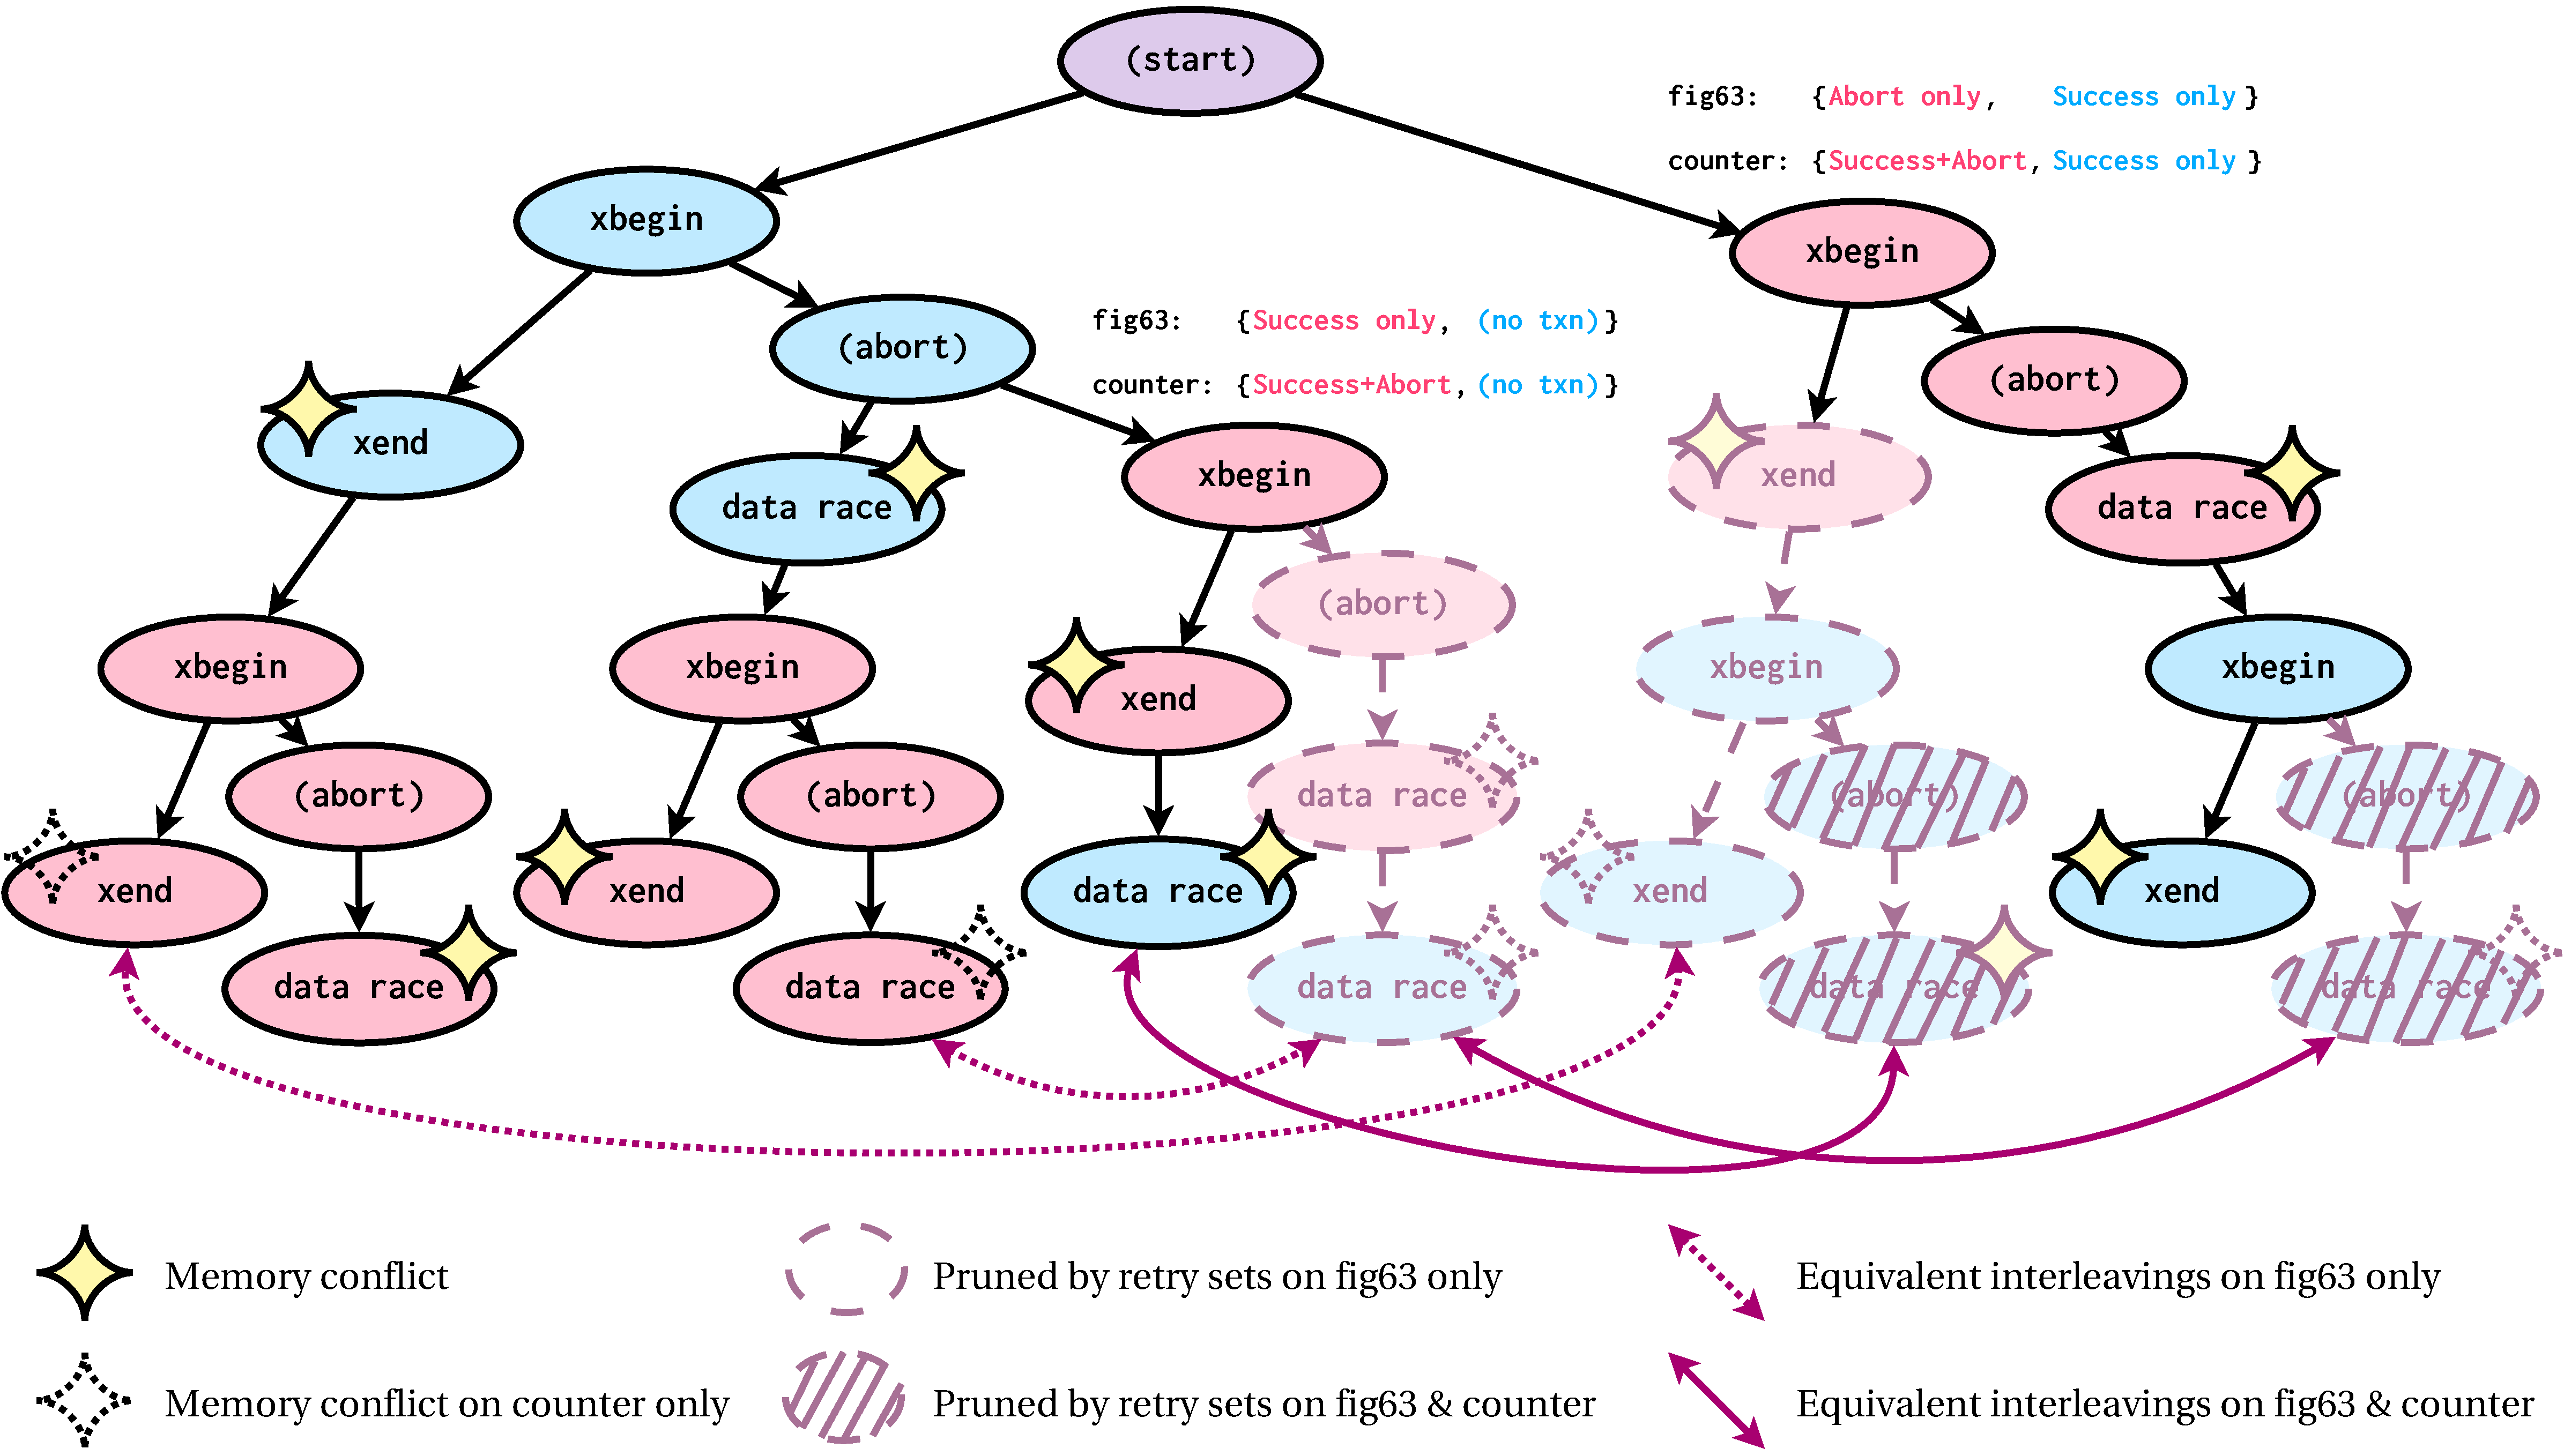
\includegraphics[width=\textwidth]{../retry-sets.pdf}
	\end{center}
\end{frame}

\begin{frame}{How good is $K,N$?}
	\begin{center}
		\small
		\begin{tabular}{c||c|c|c||c}
			{\bf test} & {\bf \#txn} & {\bf \#sync} & {\bf \#race} & {\bf max events verified} \\
			\hline
			{\tt htm2}	      & 1     & 2     & 4     & 42    \\ % 2,3
			{\tt counter}	   & 1     & 0     & 1     & 16    \\ % 2,4
			{\tt swap}	      & 1     & 4     & 8     & 52    \\ % 2,2
			{\tt fig63}	     & 1     & 0     & $K$-1 & 18    \\ % 3,2 k=3 -> 18; 2,4 -> 16
			{\tt avl\_insert}       & 1     & 2     & 7     & 20    \\ % 2,1 nb. only 5 drpps under -A -S but w/e
			% nb less than 9 on stm
			{\tt avl\_fixed}	& 1     & 2     & 9     & 24    \\ % 2,1 nb. again, only 5 under -A -S
			% nb stm takes it down from 13 to 10 races
			{\tt map\_basic}	& 1     & 4     & 13    & 36    \\ % 2,1
			% mysteriously had this at 6 at one point but ive no idea where that came from
			{\tt map\_basicer}      & 1     & 2     & 5     & 32    \\ % 2,2

			% TODO: check these again, will 2,4 even complete on mutex
			{\tt lock}({\tt spinlock})      & 1     & 2     & 4     & 28    \\ % 2,2
			{\tt lock}({\tt spin\_fixed})   & 1     & 2     & 4     & 28    \\ % 2,2 or 4,1
			{\tt lock}({\tt mutex})	 & 1     & 2     & 2     & 30    \\ % 2,3 gives 30; 2,4 would give 40
			% not putting lock_fast because it like, doesn't have a "state space" per se
		\end{tabular}
	\end{center}
	\linegap

	\begin{itemize}
		\item {\em [Abdulla '14]} reports 19 threads (??)
			\begin{itemize}
				\item {\sf filesystem(19)}: classic DPOR: 4096; (their) optimal DPOR: 64
			\end{itemize}
			% not really a quote, but their x axis from figure 9 graph, whose y axis goes up to 10k
		\item {\em [Zhang '15]} verifs up to 10 ``concurrent events'' (weak mem r/w?)
	\end{itemize}
\end{frame}

%% including this stuff in the talk now so this bonus slide is frivolous
%% TODO: slide number c.c
%\begin{frame}{Don't you need \texttt{if (mutex\_is\_locked(\&count\_lock)) \_xabort();} in that transaction on slide 42?}
%	\begin{center}
%	Yes.
%	\end{center}
%\end{frame}

%%%%%%%%%%%%%%%%%%%%%%%%%%%%%%%%%%%%%%%%%%%%%%%%%%%%%%%%%%%%%%%%%%%%%%%%%%%%%%%%
\subsection{Bibliography}

\begin{frame}{References}
	\footnotesize
	\begin{itemize}
		%\item {\bf [A., D. '52]}: T. Anderson and D. Darling.
		%	Asymptotic theory of certain ``goodness-of-fit'' criteria based on stochastic processes.
		%	Annals of Statistics, 1952.
		\item {\bf [Lamport '78]}:
			Leslie Lamport. Time, clocks, and the ordering of events in a distributed system.
			Communications of the ACM, 1978.
		\item {\bf [Godefroid '97]}: Patrice Godefroid.
			VeriSoft. A tool for the automatic analysis of concurrent reactive software. CAV 1997.
		%\item {\bf [Holzmann '97]}: The model checker SPIN. TOSE 1997.
		\item {\bf [Engler '03]}: Dawson Engler and Ken Ashcraft.
			RacerX: effective, static detection of race conditions and deadlocks. SOSP 2003.
		\item {\bf [O'Callahan '03]}: Robert O'Callahan and Jong-Deok Choi.
			Hybrid dynamic data race detection. PPoPP '03.
		\item {\bf [Flanagan '05]}: Cormac Flanagan and Patrice Godefroid. Dynamic partial-order reduction for
			model checking software. POPL 2005.
		\item {\bf [Musuvathi '08]}: Madanlal Musuvathi et al. Finding and Reproducing Heisenbugs in Concurrent
			Programs. OSDI 2008.
		\item {\bf [Yang '08]}: Yu Yang et al. Efficient stateful DPOR. SPIN 2008.
		\item {\bf [Klein '09]}: Gerwin Klein et al. seL4: formal verif. of an OS kernel. SOSP 2009.
	\end{itemize}
\end{frame}
\begin{frame}{References}
	\footnotesize
	\begin{itemize}
		%\item {\bf [Burckhardt '10]}: A randomized scheduler with probabilistic guarantees of finding bugs. ASPLOS 2010.
		\item {\bf [Simsa '12]}: Jiri Simsa. Runtime Estimation and Resource Allocation for
			Concurrency Testing. Tech report (CMU-PDL-12-113). December 2012.
		\item {\bf [Blum '12]}: Ben Blum. Landslide: Systematic Dynamic Race Detection in Kernel Space.
			MS thesis (CMU-CS-12-118). May 2012.
		\item {\bf [Kasicki '12]}: Baris Kasicki. Data races vs. data race bugs: telling the difference with Portend. ASPLOS '12.
		\item {\bf [Simsa '13]}: Systematic and Scalable Testing of Concurrent Programs.
			Ph.D. thesis (CMU-CS-13-133). December 2013.
		%\item {\bf [Coons '13]}: Katherine Coons et al. Bounded POR. OOPSLA 2013.
		\item {\bf [Abdulla '14]}: Parosh Abdulla et al. Optimal DPOR. POPL 2014.
		\item {\bf [Matsakis '14]}: Nicholas Matsakis et al. The Rust Language. HILT 2014.
		\item {\bf [vamsikc '14]}: leveldb-tsx. https://github.com/vamsikc/leveldb-tsx/, 2014.
		%\item {\bf [Huang '15]}: Jeff Huang. Stateless MCing concurrent programs with maximal causality reduction. PLDI '15.
		\item {\bf [Jensen '15]}: Stateless MCing of Event-Driven Applications. OOPSLA 2015.
		\item {\bf [Dehesa-Azuara '16]}: Hardware transactional memory with intel's TSX.
			http://www.contrib.andrew.cmu.edu/\textasciitilde{}mdehesaa/, 2016.
	\end{itemize}
\end{frame}

\end{document}
